\chapter{Monte Carlo Methods}
\index{Monte Carlo Methods}
\thispagestyle{empty}

Monte Carlo methods account for a large set of methods that incorporate random number generation in solving a problem numerically. Monte Carlo algorithms are in wide use in many different search algorithms, especially in cases where minimum energy (or cost) is hard to define. In the case of a parameter optimization in a smooth energy landscape, finding a global minimum, or at least an exceptionally good local minimum is a well studied problem, and there are many ways to attack this problem. Problems arise when the parameter space is not continuous, or the energy landscape is not smooth, in which then small perturbations in initial conditions lead to different local minima. One example that might be given is a chess opening, \newgame
\mainline{1.e4 e5}.

\begin{center}
\showboard
\end{center}

This is the \textbf{open game} opening, a mainstream opening in chess. We can think of the chess game as a statistical system where all configurations of the chess pieces are states that a game can be in. It is evident that a system can't jump from any state to another, for example, a bishop in white squares can't be in a black square \footnote{Except for the exceptional case where a promoted pawn is chosen to be a second bishop of black tiles.} 
, but still, there are still a huge amount of positions (or states) available for the game to be in and a game is actually how this state has evolved into a checkmate or a draw. In this particular game, the white has a many choices, for example, \mainline{2.f4 ...} is  called a \textbf{King's Gambit}, white offers a pawn in exchange of a positional advantage. 

\begin{center}
\showboard
\end{center}
\newgame
This one of the examples where another game or state, such as  \mainline{1.e4 e5 2.d4...} seems to be a similar one, though for the player, this offers a very different set of opportunities than a King's Gambit would offer.

\begin{center}
\showboard
\end{center}

There isn't a straightforward way to reach the most advantageous state in a chess game, that's what makes it a game. But if this is the case, there is a hard time for a deterministic machine to make a move, since optimization algorithms such as gradient descent depend on the fact that small changes in parameters would lead to small changes in performance, it is evident this is not the case here. Or, one might argue rightly that our visual perception is a bad informant of a norm in all state space, since states here are not in a space, but are in a tree (or a graph) of recursively branching moves, all of the tips being checkmates of draws.  

So an artificial intelligence  \footnote{Let's assume that here that it is an AI that all previous knowledge of chess, openings, plays... are erased, an AI tabula rasa.} would go for choosing moves, walk the portion of the tree of states that is $ n $ moves away from the initial state, and calculate its advantage for every play. The deeper the AI goes in its search, better moves it will eventually find, but most of the time it takes a huge amount of time to traverse the tree of positions, so most game engines use a method called \textbf{Monte Carlo Tree Search}, in which the way that the tree is explored is randomized. The game tree grown in the memory with these random explorations are then used to make the best move available to the AI. This gives the AI a deeper search for a given amount of time, and a relatively good move. Randomized tree search is even more popular in games like Go, where the amount of moves available to the user is much greater.

So one doesn't lack motivation in order to incorporate random guessing in searching for an optimum state, especially in cases where the complexity is great enough to veil any deterministic ways to search for such minimum. Chess is not the perfect example here, but financial systems, biological systems, manufacturing variations are systems where Monte Carlo methods are proven effective.    

\section{Monte Carlo Methods in Statistical Systems}

Another area where Monte Carlo methods are preferable is statistical systems, where thermal agitation can't be handled deterministically. The most popular algorithm in this genre is the \textbf{Metropolis–Hastings algorithm} \cite{metropolis}, and it is the algorithm that this paper will focus on. First a particular example about Ising spins is presented, than the algorithm is generalized step by step. 

\subsection{Metropolis Algorithm on a 2D Ising Chain}

Let us assume that there is a 2D spin glass of random spin distribution and size $ 50\times 50 $. Here, spins up and down are visualized as black and white squares.

	\begin{figure}[H]
	\center
	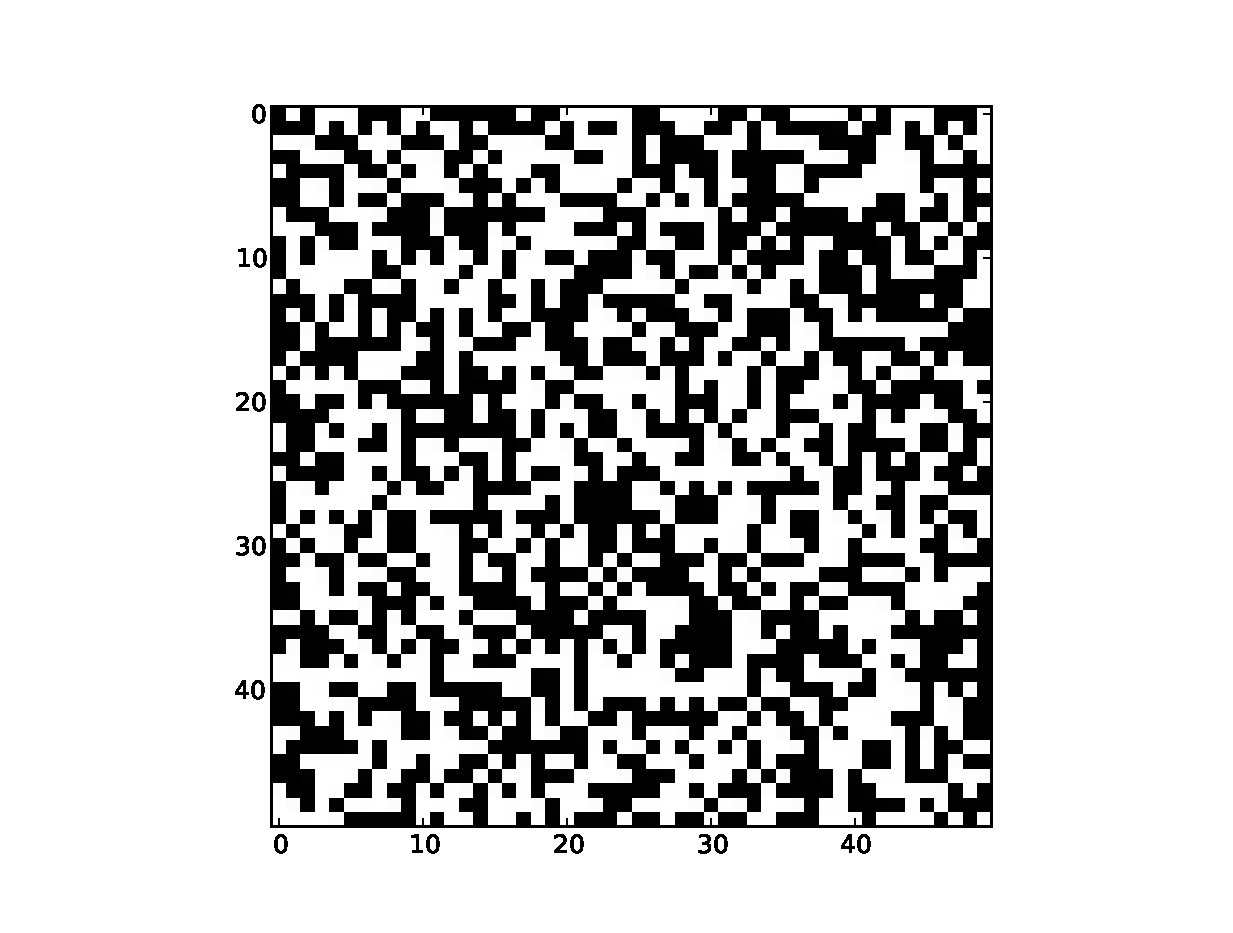
\includegraphics[width=0.5\linewidth]{fig/spins.eps}
	\label{fig:spins}
	\caption[Randomly distributed 2D Ising spins]{Randomly distributed 2D  Ising spins. In this paper, spin systems will be visualized like this.}
	\end{figure}
	
This configuration can be attributed to an energy value. If individual spins are denoted as $ \sigma_{i} \in {-1,1} $, \footnote{I avoided double indices for the sake of simplicity} then the Ising Hamiltonian can be loosely formulated in this way:

\begin{equation}
\label{eq:hamiltonian}
\mathcal{H} = - J \sum\limits_{\left\langle ij \right\rangle} \sigma_{i} \sigma_{j} -h \sum\limits_{i}\sigma_{i}
\end{equation}
	
where $ \sigma_{i}$ is an individual spot on the 2D lattice, and the first sum is over spins where spin i and spin j are nearest neighbours. 

So, if a spin is up, every spin that is down in its vicinity contributes $ -J $ to the energy, and every spin that is up contributes $ J $ to its energy.  

A non-degenerate system that is in thermal equilibrium with its surroundings has an probability of occupying a state with energy $ E_i $ of

\begin{equation}
\label{eq:boltzmannprob}
p(E_i) = \frac{e^{-\beta E_i}}{Z(\beta)}
\end{equation}

where $ Z(\beta) $ is the partition function. In our case, Equation \eqref{eq:boltzmannprob} is simpler:

\begin{equation}
\label{eq:sinlespinboltzmann1}
p_1 = \frac{e^{-\beta E_1}}{e^{-\beta E_1}+e^{-\beta E_{-1}}}
\end{equation}

\begin{equation}
\label{eq:sinlespinboltzmann2}
p_{-1} = \frac{e^{-\beta E_{-1}}}{e^{-\beta E_1}+e^{-\beta E_{-1}}}
\end{equation}

since there are only two states for a single spin to occupy. So, if one only observes this particular spin only from the fact that there is an ongoing thermal agitation, it will occupy the energetic state with probability $ p_1 $. 

The Metropolis algorithm uses this fact. For a spin, if the rotated spin results in a lower energy configuration, this configuration is preserved. If the rotated spin results in a higher energy configuration, there is still a chance that this configuration is attained, since the thermal vibrations can contribute for that, and this probability is 

\[p_{\text{flip}} = e^{-\beta \Delta E}\] 

where $ \Delta E $ is the energy change required to flip the spin. One can guess that such an algorithm will eventually reach down to states that flux of spins pumped up to an antisymmetric configuration will be equal to the flux of spins that lose energy by attaining a symmetric configuration. Here, $ \beta $ is a parameter that can be tuned, it is $ 1/k_B T $. When this equilibrium is reached, the macroscopic variables of the system is considered to be unchanging, and after the difference in consecutive calculations of the macroscopic variable is below some value, it can be used as is. 

So if one writes the steps of the algorithm:
\begin{enumerate}
\item Create a random configuration of spins.
\item Do the following for $ \Pi $ times:
	\begin{enumerate}
	\item Choose a random spin.
	\item Calculate the energy change, $ \Delta E $.
		\begin{enumerate}
		\item If $ \Delta E < 0 $, then preserve the orientation of the spin.
		\item If $ \Delta E > 0 $, then generate a random number $ \alpha \in (0,1) $
			\begin{enumerate}
			\item If $ \Delta E < \alpha $, then preserve the orientation of the spin.
			\item If $ \Delta E > \alpha $, then flip the spin.
			\end{enumerate}
		\end{enumerate}
	\end{enumerate}
\item Calculate $ M $ , magnetization, if the value fo the magnetization is within error bounds, get out of the algorithm. If not, continue to do so until the error is within bounds.  
\end{enumerate}

This is how the algorithm is implemented for a 2D Ising spin configuration. The 3D case is rather easy to guess, it follows the same logic.

\section{Metropolis Algorithm for an Arbitrary Statistical System}

The aim in this project is not to make numerical calculations for various systems, such as 1D, 2D, 3D Ising chains. I'd rather like to generalize the Metropolis Algorithm in such a way that it can be implemented for various other statistical systems also. The aim is to code a modular Metropolis engine that a set of statistical systems can be implemented to the code, by using a backbone that is applicable to all of them. 

I will explain the generalization procedure by applying it to the Ising case. What Metropolis algorithm does is the following. It takes a randomized \textbf{configuration}, and for a single \textbf{element} of the statistical ensemble.  hen either from a function that calculates the energy difference, or by merely calculating the energies of the configurations and subtracting them, an energy difference $ \Delta E $ is calculated. Then, the probabilities for every state this individual can be in is calculated, from a temperature and energy dependent \textbf{probability distribution}. Then, a new configuration is selected from the pool, depending on the probabilities of them. This loop is initiated for $ \Pi $ times, after macroscopic variables are calculated, and after these microscopic variables are settled, the algorithm quits. 

With this reasoning, we can think of the following objects and functions for an arbitrary algorithm.
 
\begin{enumerate}
\item Parameters ($ \beta $ , $ J $ , $ k $)
\item An ensemble definition ($ N\times N $ spin system)
\item An element definition  (A spin, up or down)
\item An energy definition with respect to some parameters (Hamiltonian \eqref{eq:hamiltonian})
\item A probability distribution with respect to some parameters (Boltzmann distribution)
\item Macro parameters to calculate from the ensemble (Magnetization)
\item If any, an external condition applied via changing parameters. (There were none)
\end{enumerate}

By generalizing this, a Metropolis algorithm may be used for any statistical system with considerable modularity. For example, a gas can also be simulated with this approach. 

So, this approach can be implemented as the following. There  can be classes \textbf{Ensemble} and \textbf{Element} , in which the ensemble houses a list of elements. 

\section{Ising Spins as an Example}

In order to exemplify this modular approach, a system of $ 20 \times 20 $ spins were exposed to this algorithm. The class of \emph{SpinGlass} houses all functions that incorporate for every action taken in the ensemble. Methods defined in the class will calculate the energy or the energy difference, the element list, the parameters, and the whole process of selecting an element, calculating the energy difference for it to be rotated, and proceed accordingly. 

After each parameter change, which is triggered with a condition satisfied, the magnetization $ M $, is calculated. The temperature $ \beta $ is swept from 0.1 to 1.05 and the following are the plot of magnetization versus the temperature. In this trial, the values for the coefficients are selected to be $ J=1 $, $ h=0 $, for simplicity. 

\begin{figure}[H]
\center
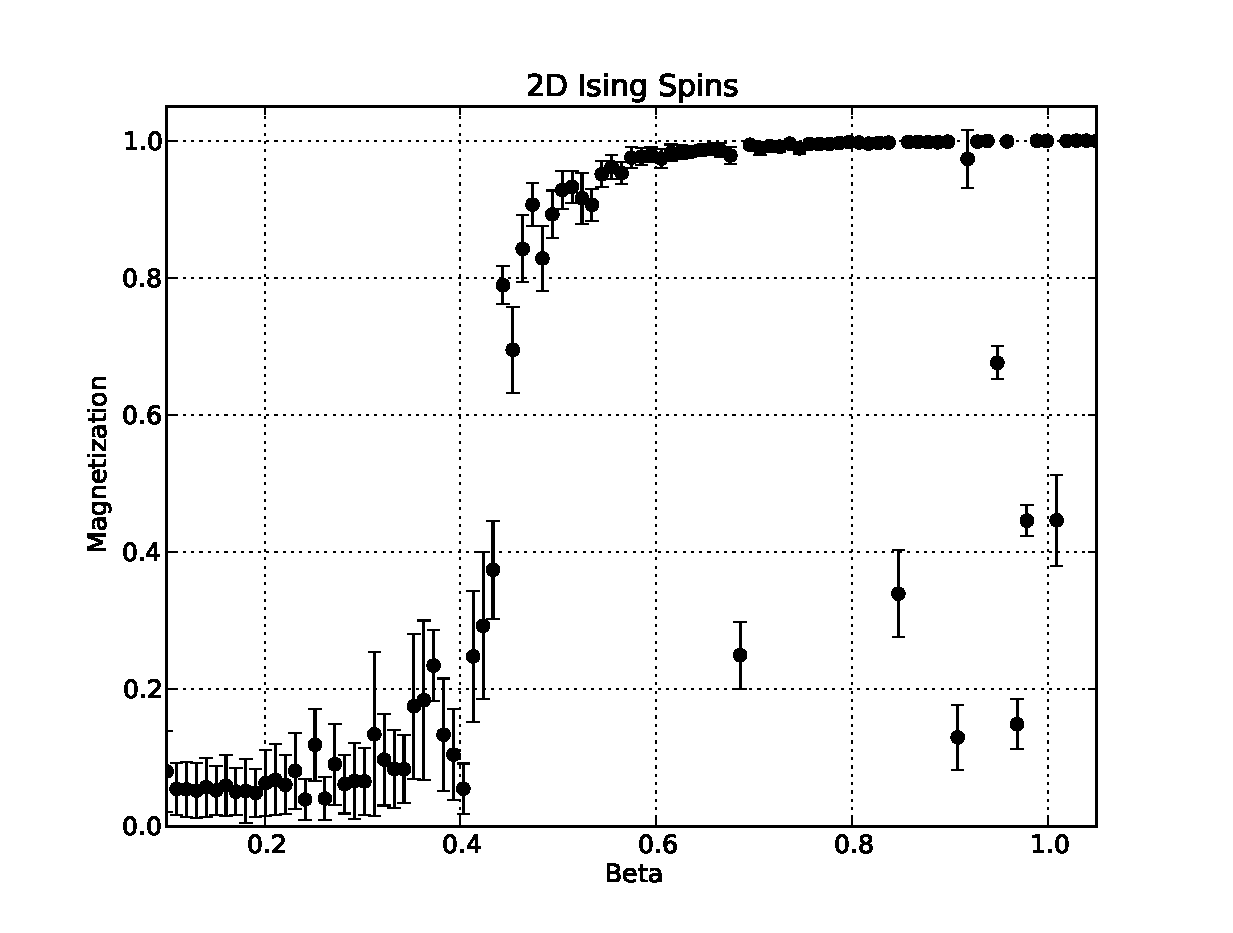
\includegraphics[width=\linewidth]{fig/20/ploterr.eps}
\label{fig:400spins}
\caption[The dependence of magnetization $ M $ due to the temperature, $ \beta $.]{The dependence of magnetization $ M $ due to the temperature, $ \beta $. The error bars correspond to the standard deviations and the dots correspond to the mean of the data set taken for that $ \beta $ value. The deviations from the orderly phase are from the fact that the standard deviation may turn out to be low though the algorithm hadn't converged.}
\end{figure}

\begin{figure}[ht]
\centering
\subfigure[$ \beta=0.1 $]{
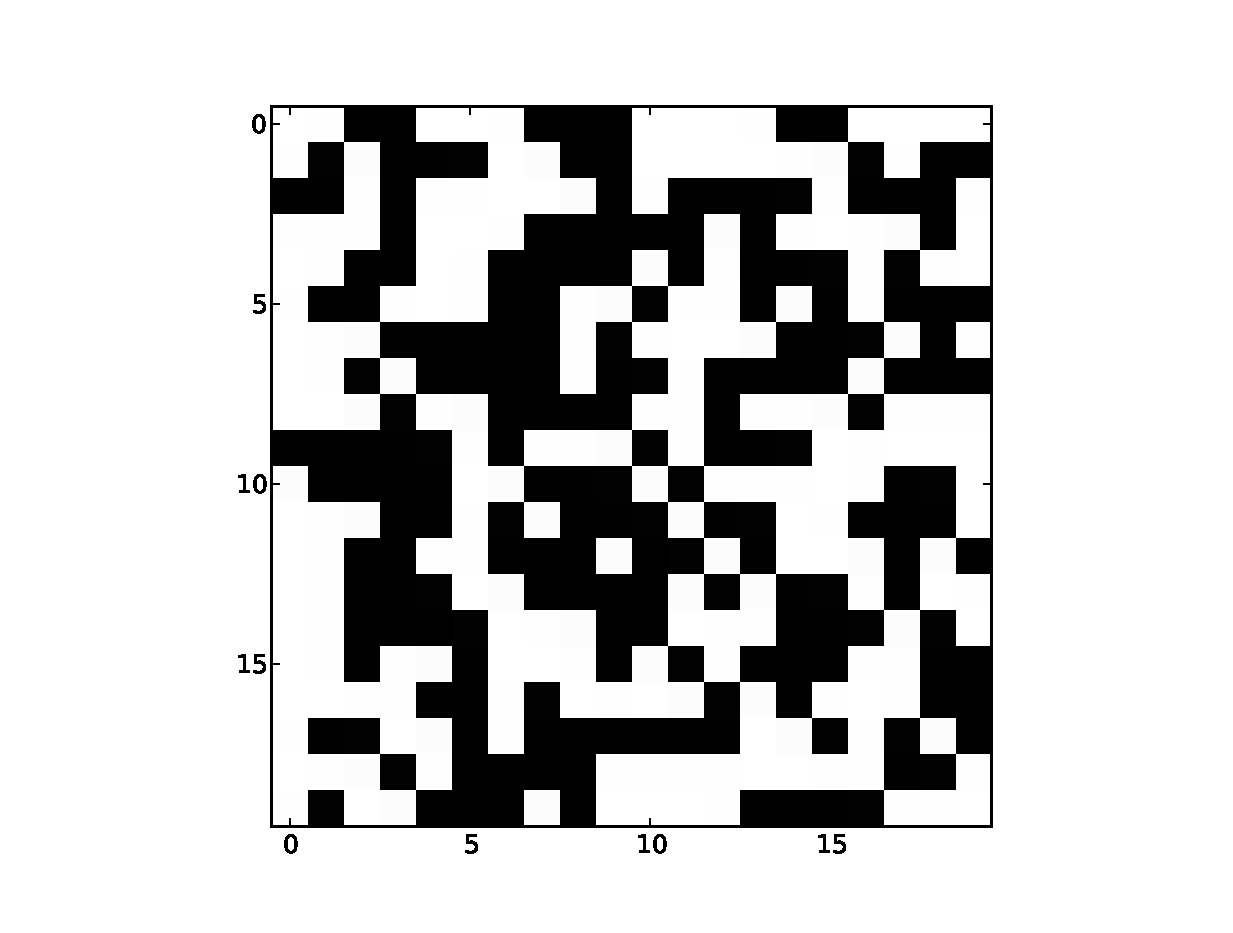
\includegraphics[width=0.3\linewidth]{fig/20/1.eps}
\label{fig:s1}
}
\subfigure[$ \beta=0.15 $]{
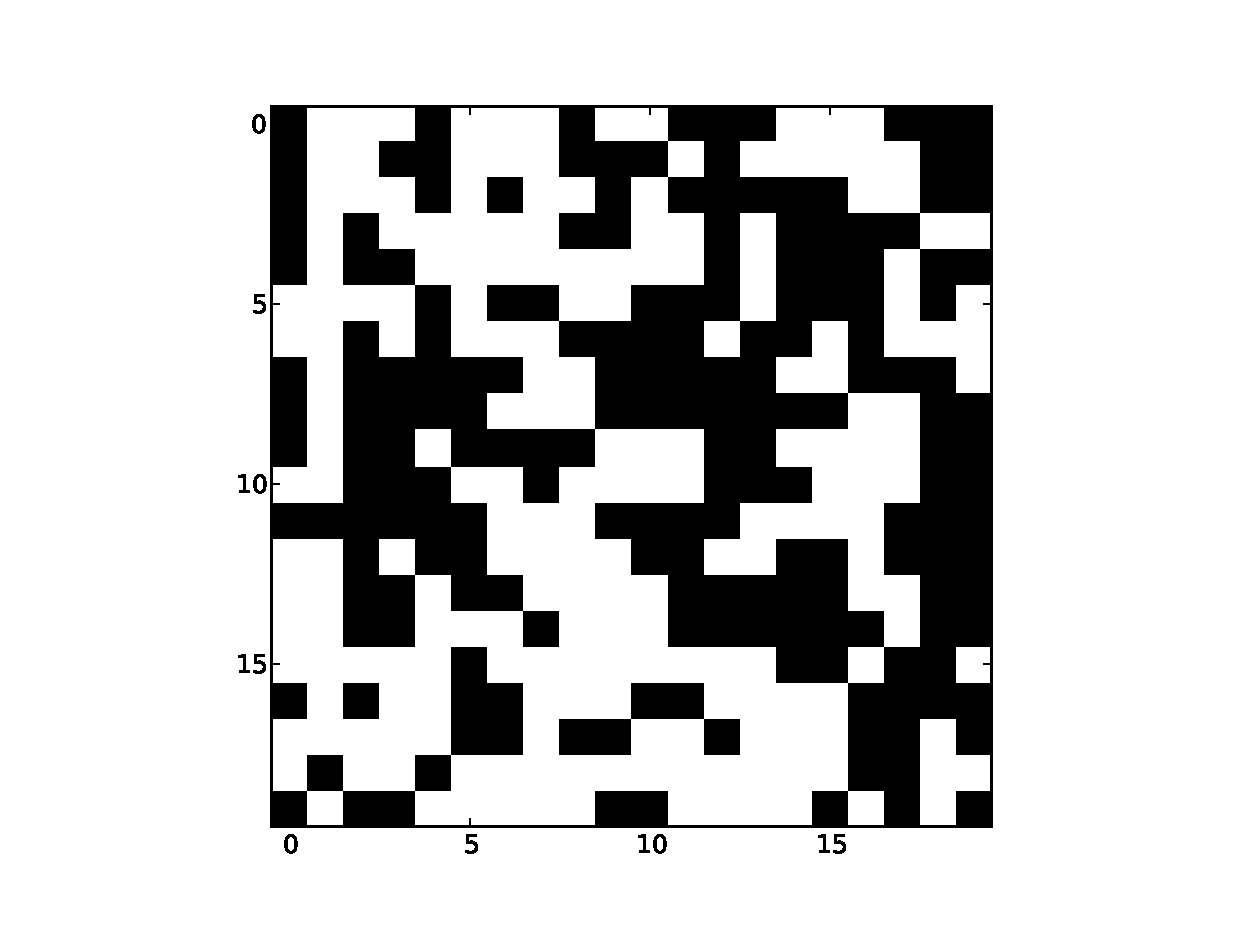
\includegraphics[width=0.3\linewidth]{fig/20/2.eps}
\label{fig:s2}
}
\subfigure[$ \beta=0.2 $]{
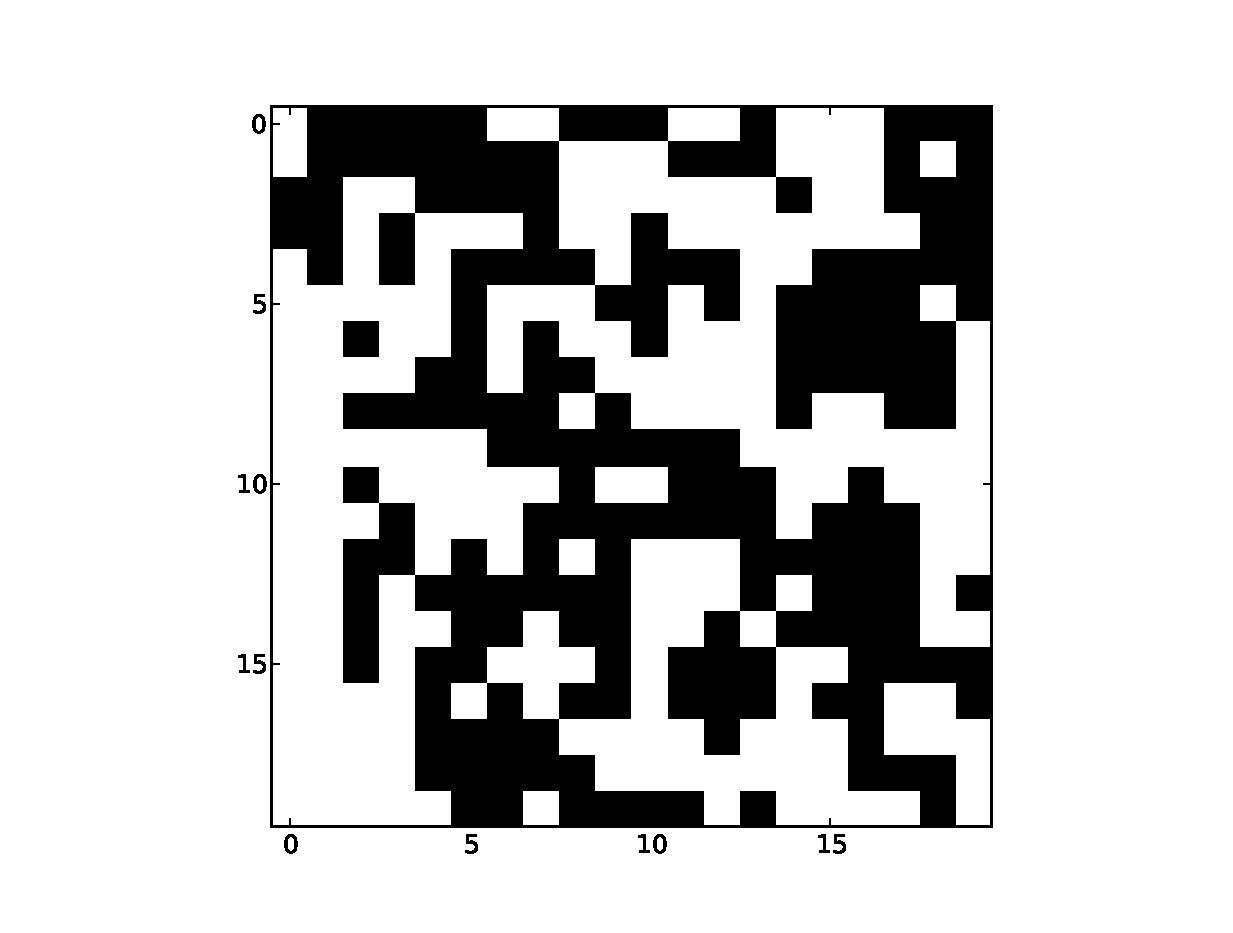
\includegraphics[width=0.3\linewidth]{fig/20/3.eps}
\label{fig:s3}
}
\\
\subfigure[$ \beta=0.25 $]{
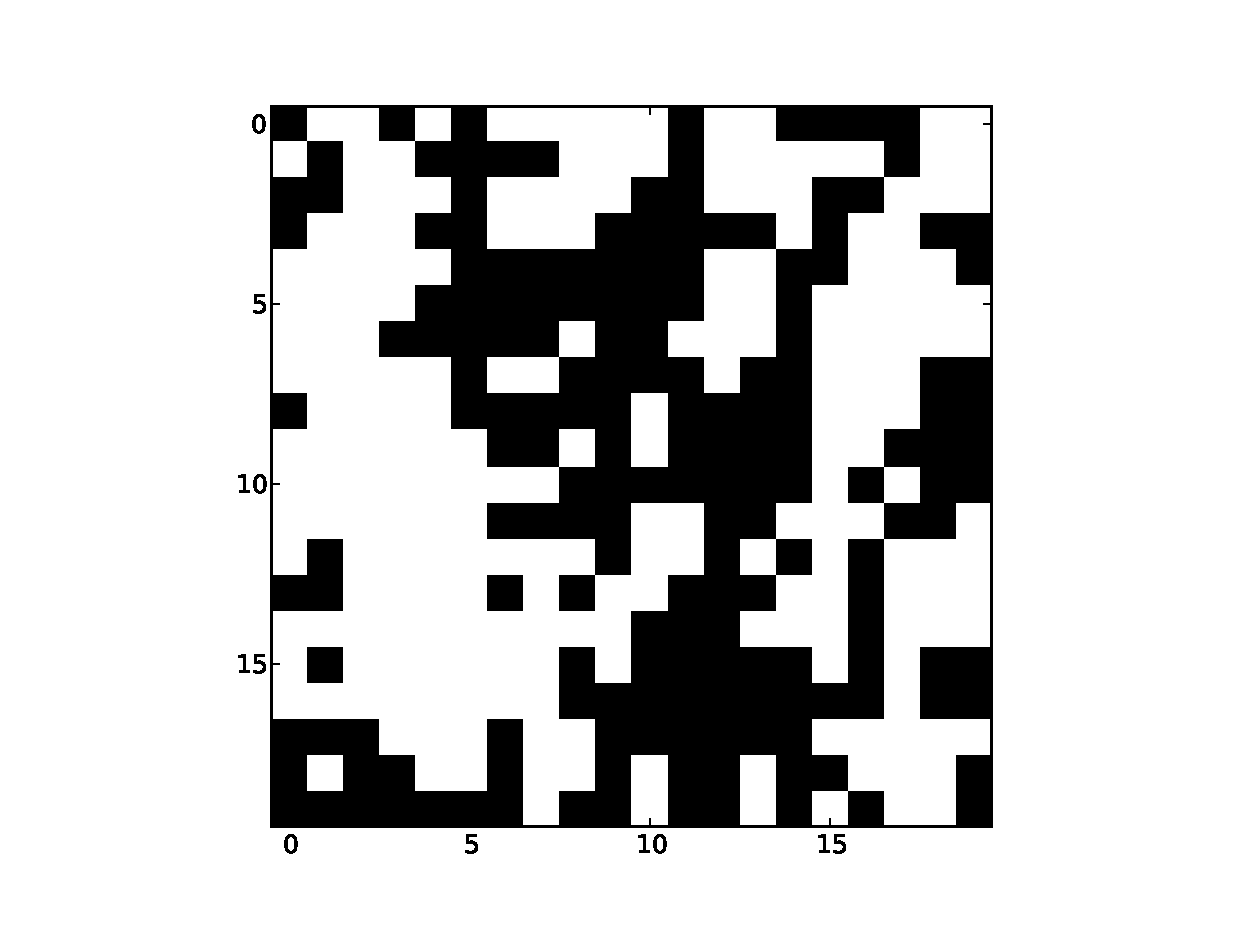
\includegraphics[width=0.3\linewidth]{fig/20/4.eps}
\label{fig:s4}
}
\subfigure[$ \beta=0.30$]{
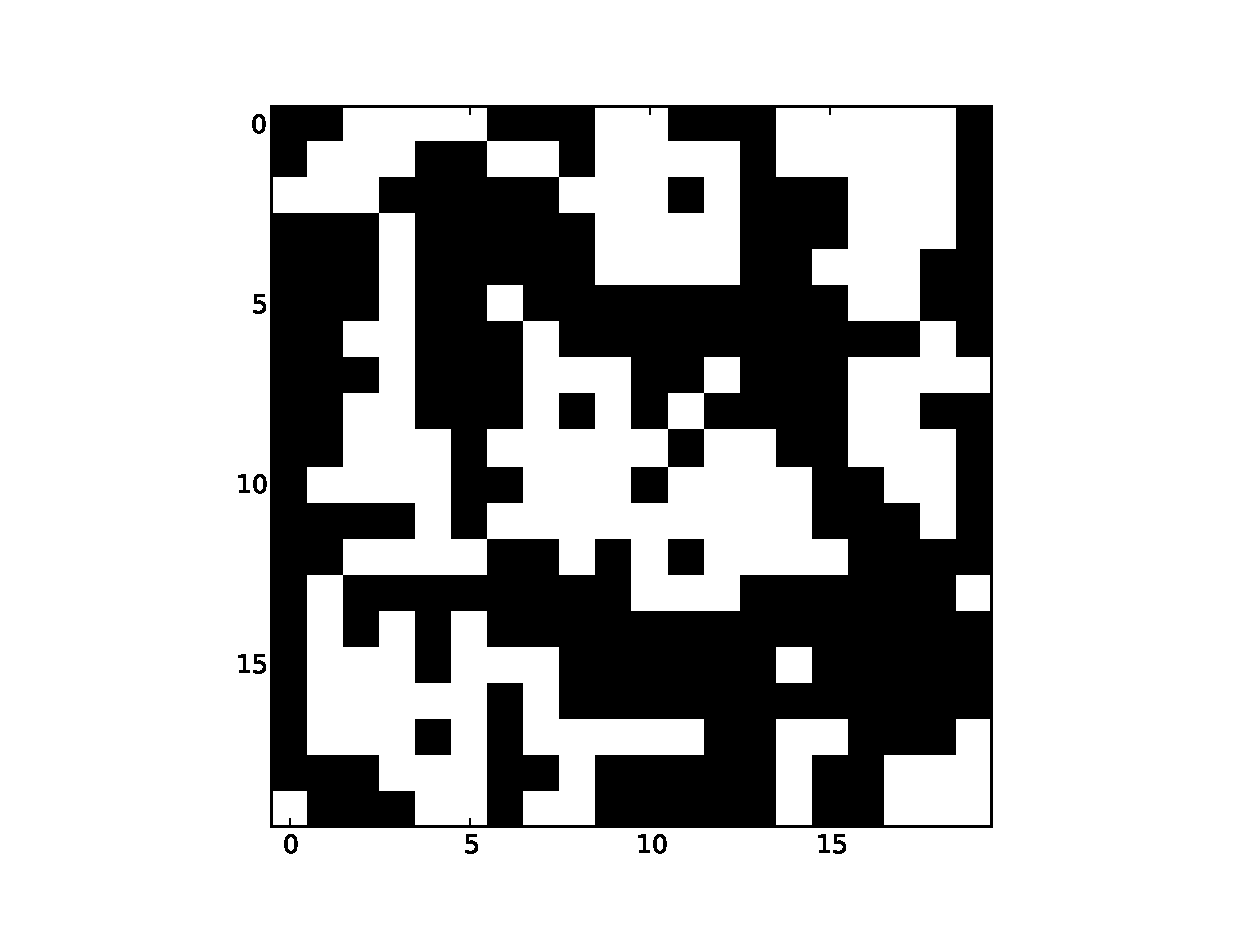
\includegraphics[width=0.3\linewidth]{fig/20/5.eps}
\label{fig:s5}
}
\subfigure[$ \beta=0.35$]{
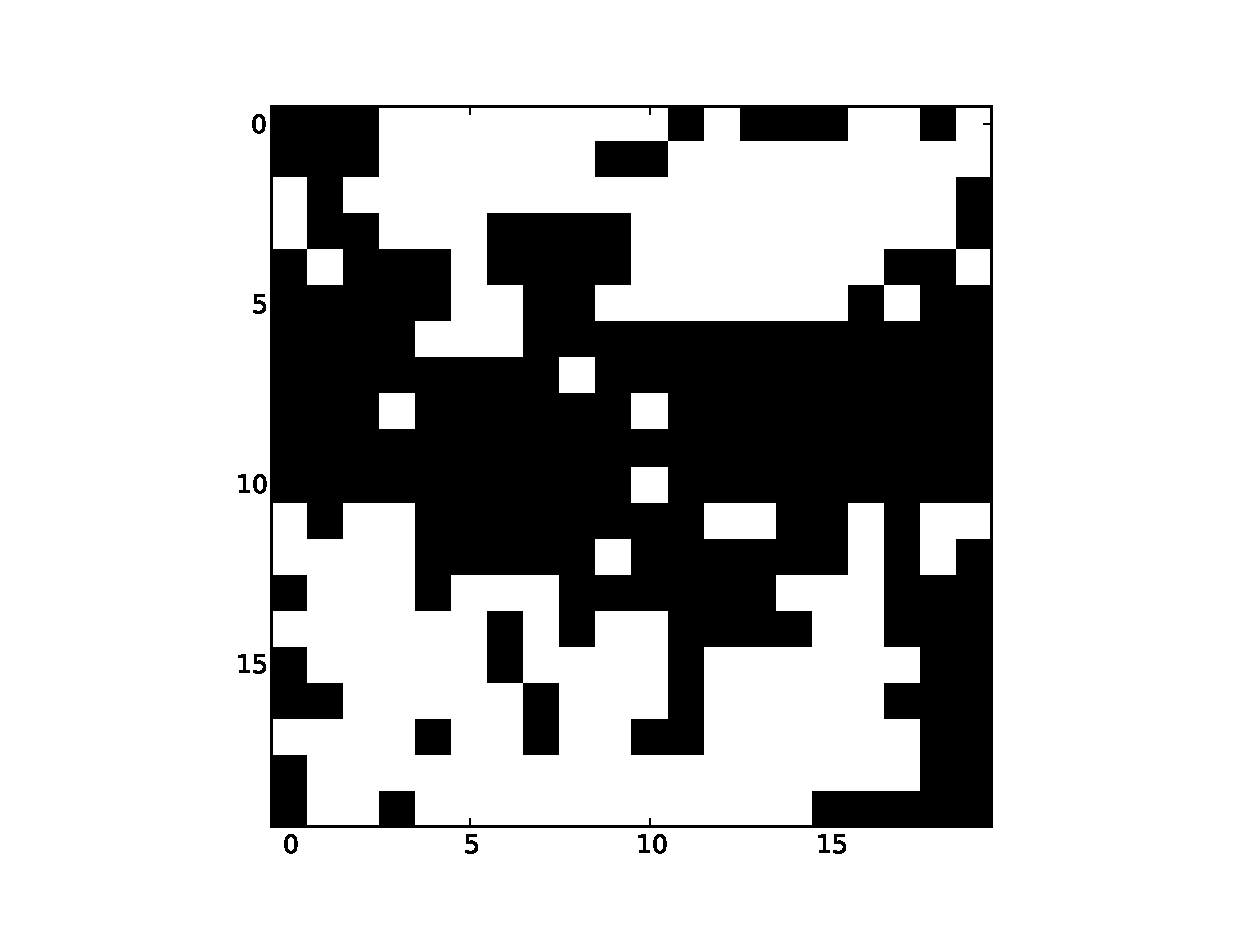
\includegraphics[width=0.3\linewidth]{fig/20/6.eps}
\label{fig:s6}
}\\

\subfigure[$ \beta=0.40$]{
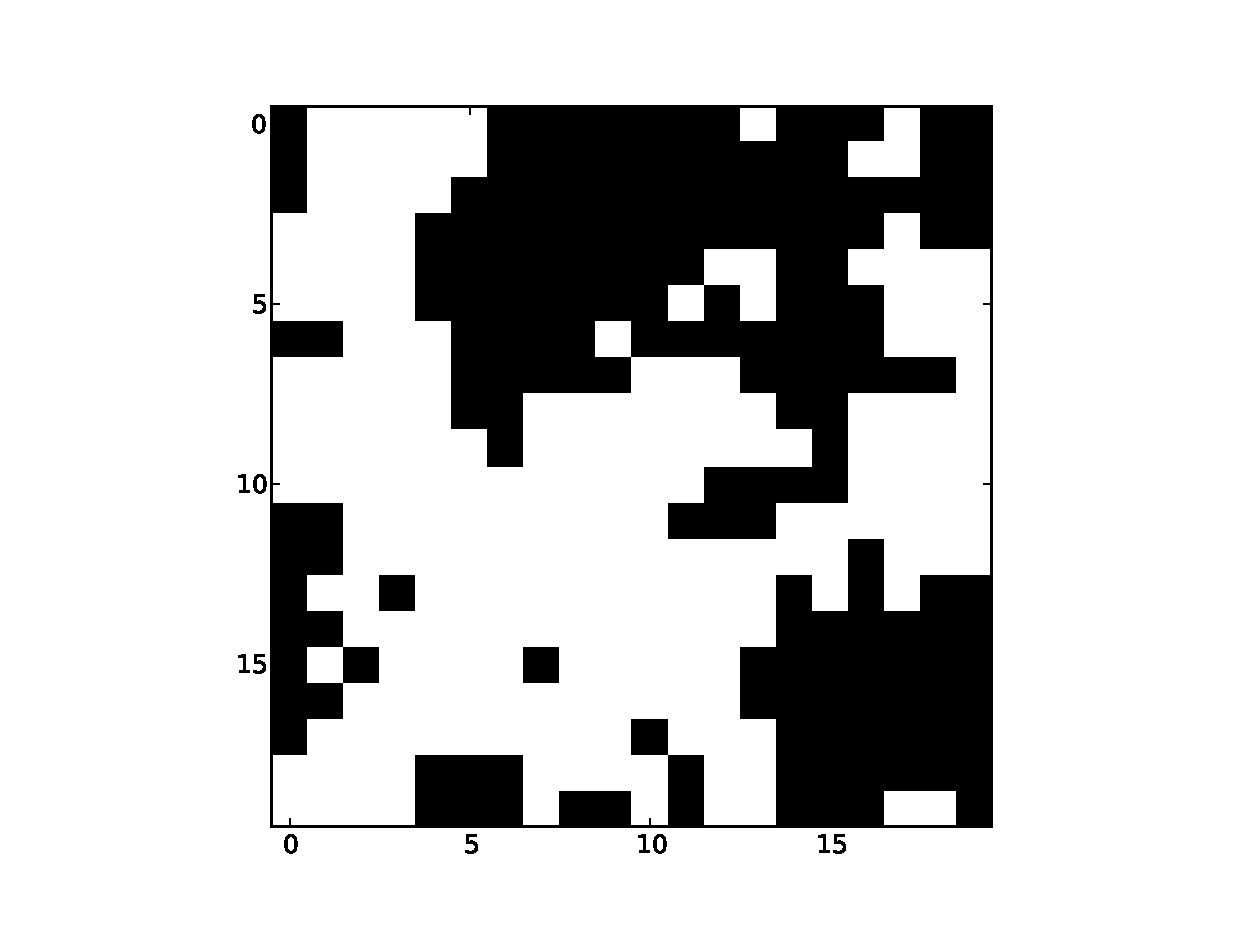
\includegraphics[width=0.3\linewidth]{fig/20/7.eps}
\label{fig:s7}
}
\subfigure[$ \beta=0.45 $]{
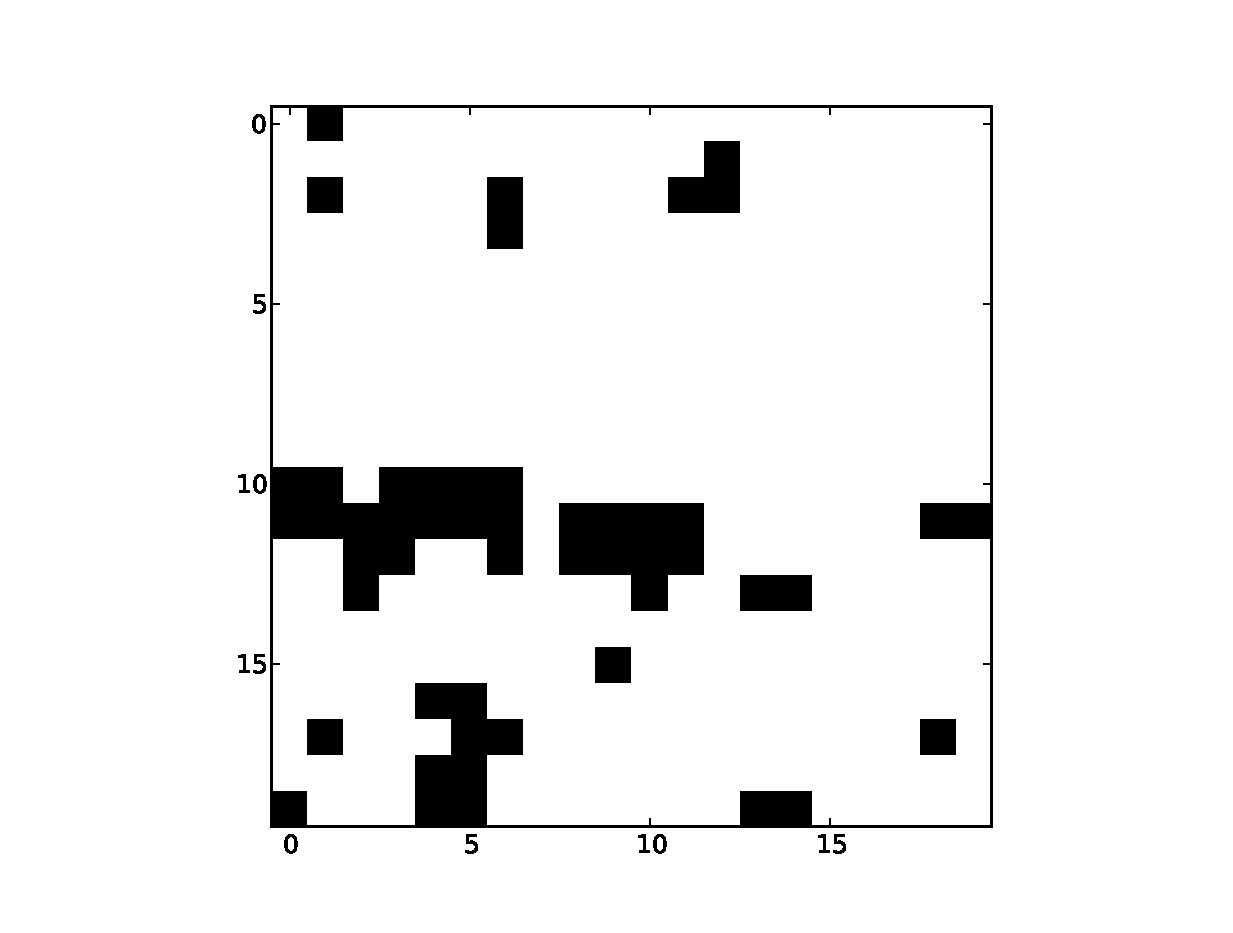
\includegraphics[width=0.3\linewidth]{fig/20/8.eps}
\label{fig:s8}
}
\subfigure[$ \beta=0.50$]{
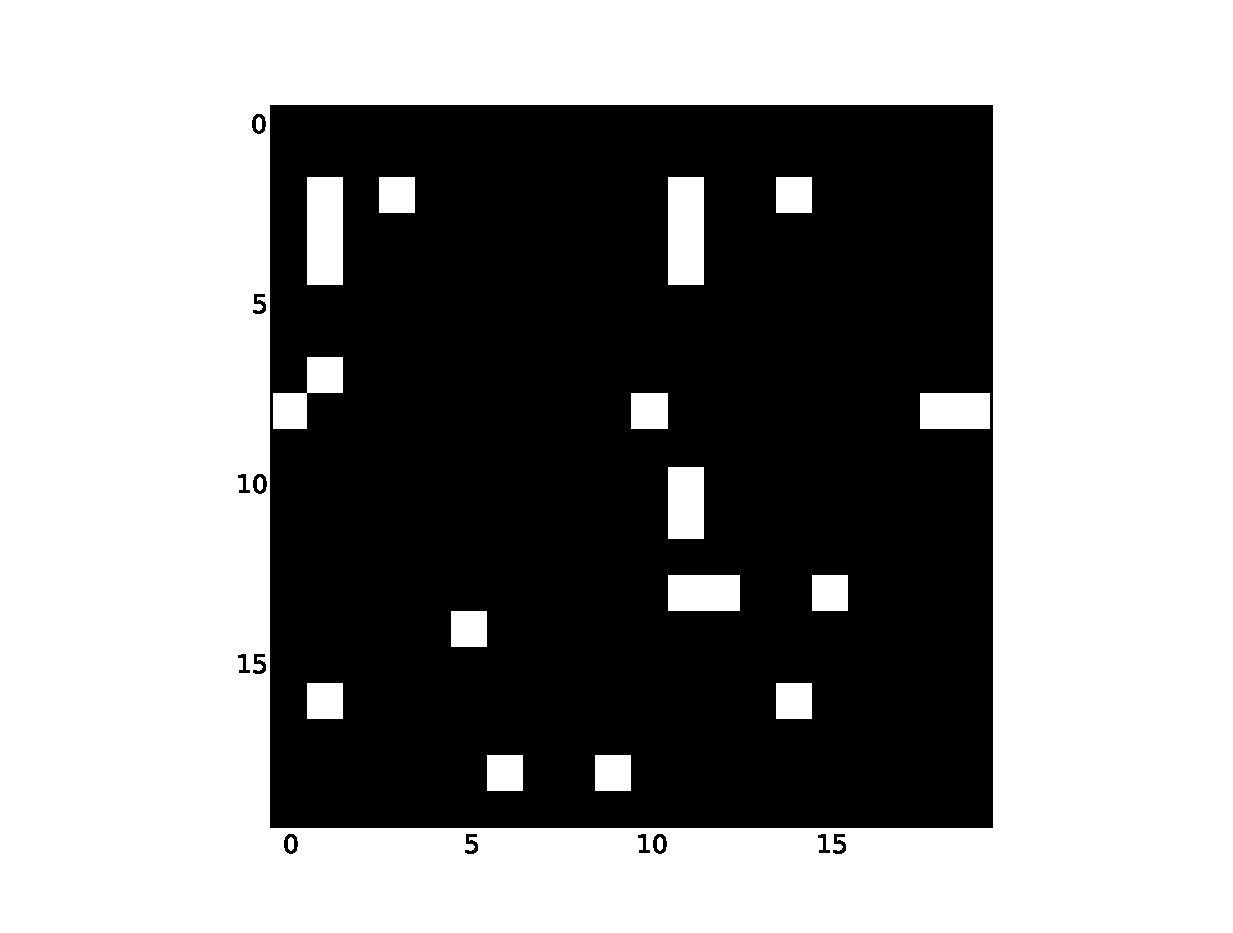
\includegraphics[width=0.3\linewidth]{fig/20/9.eps}
\label{fig:s9}
}\\

\subfigure[$ \beta=0.55$]{
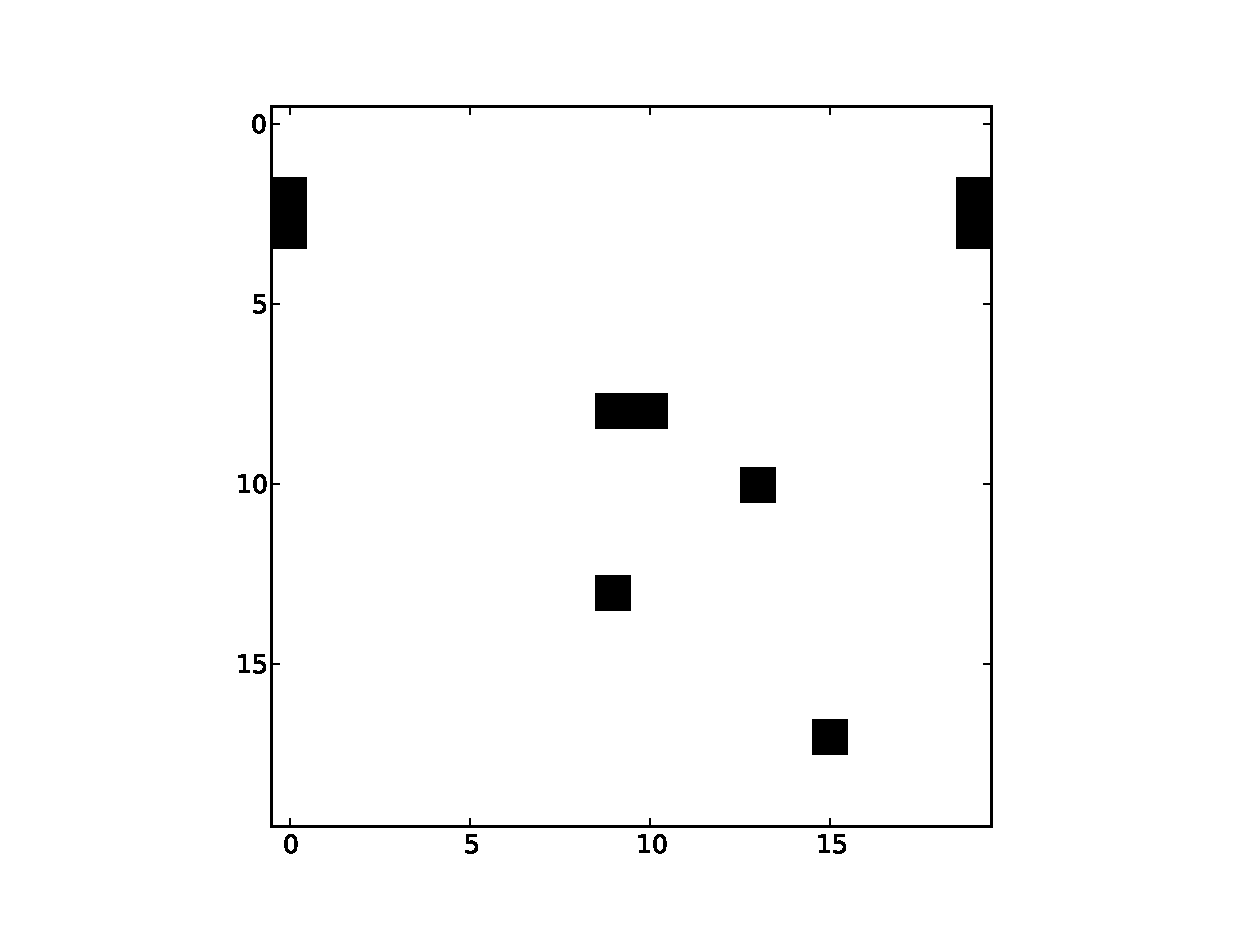
\includegraphics[width=0.3\linewidth]{fig/20/10.eps}
\label{fig:s10}
}
\subfigure[$ \beta=0.60$]{
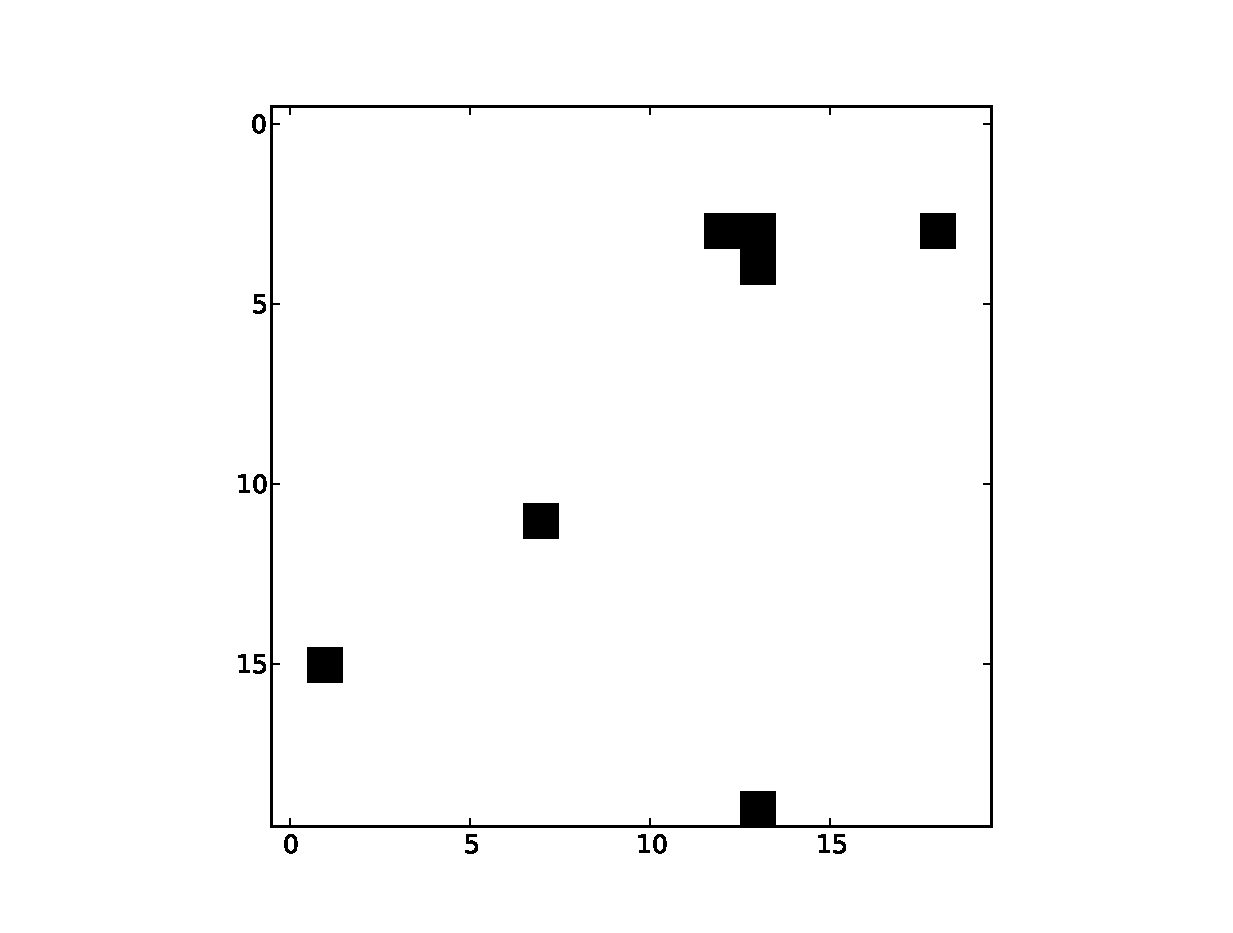
\includegraphics[width=0.3\linewidth]{fig/20/11.eps}
\label{fig:s11}
}
\subfigure[$ \beta=0.65$]{
\includegraphics[width=0.3\linewidth]{fig/20/12.eps}
\label{fig:s12}
}\\


\subfigure[$ \beta=0.70$]{
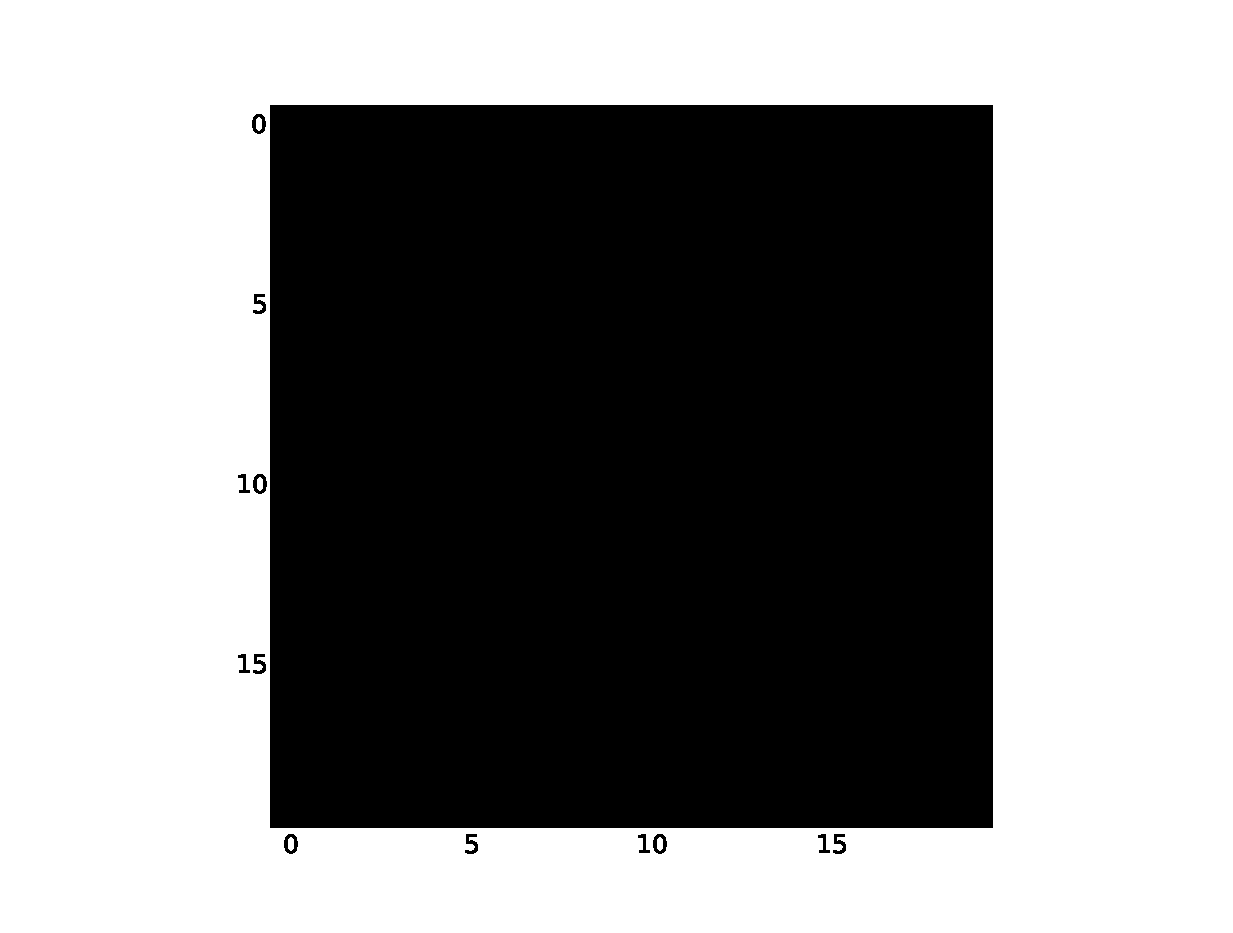
\includegraphics[width=0.3\linewidth]{fig/20/13.eps}
\label{fig:s13}
}
\subfigure[$ \beta=0.75$]{
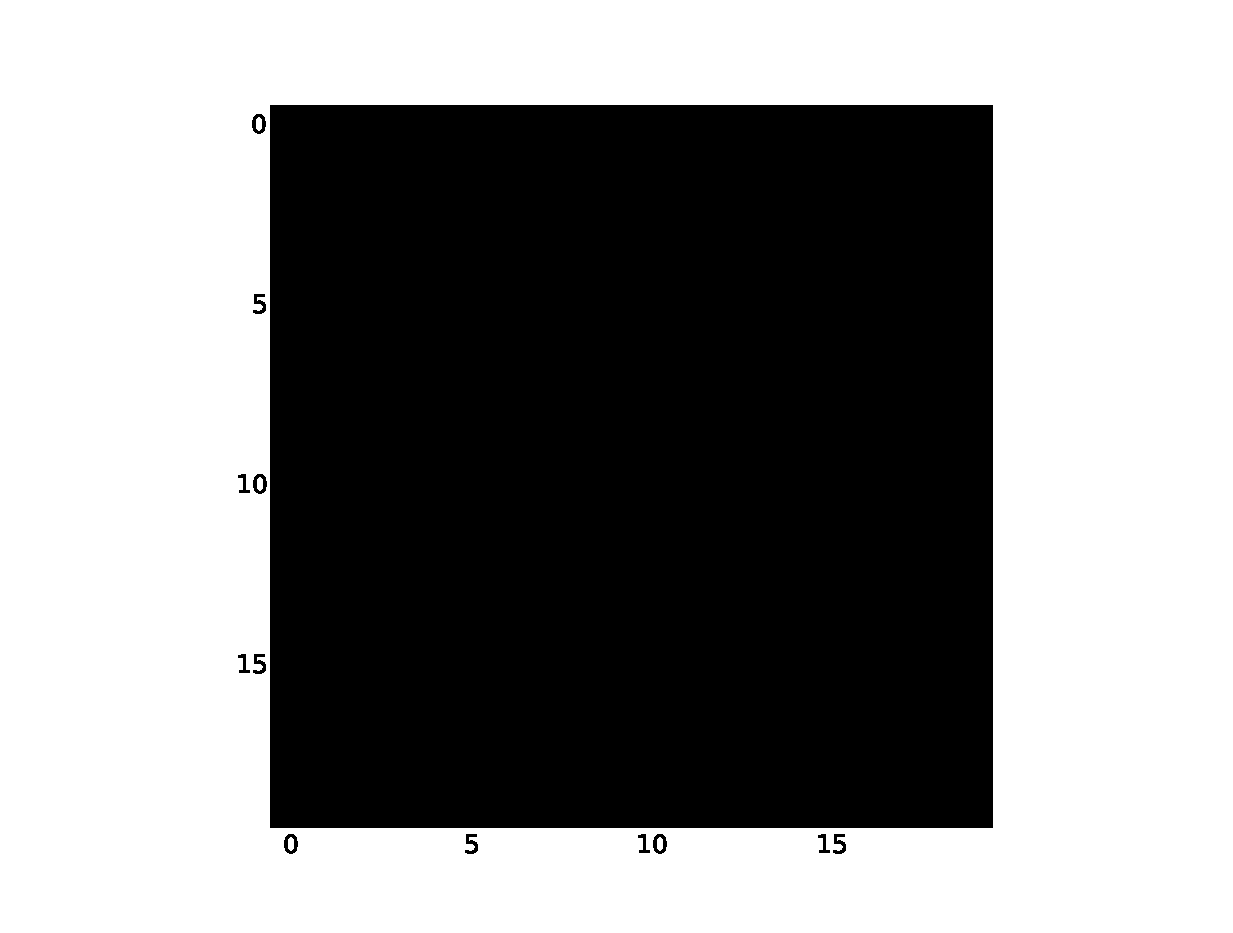
\includegraphics[width=0.3\linewidth]{fig/20/14.eps}
\label{fig:s14}
}
\subfigure[$ \beta=0.80$]{
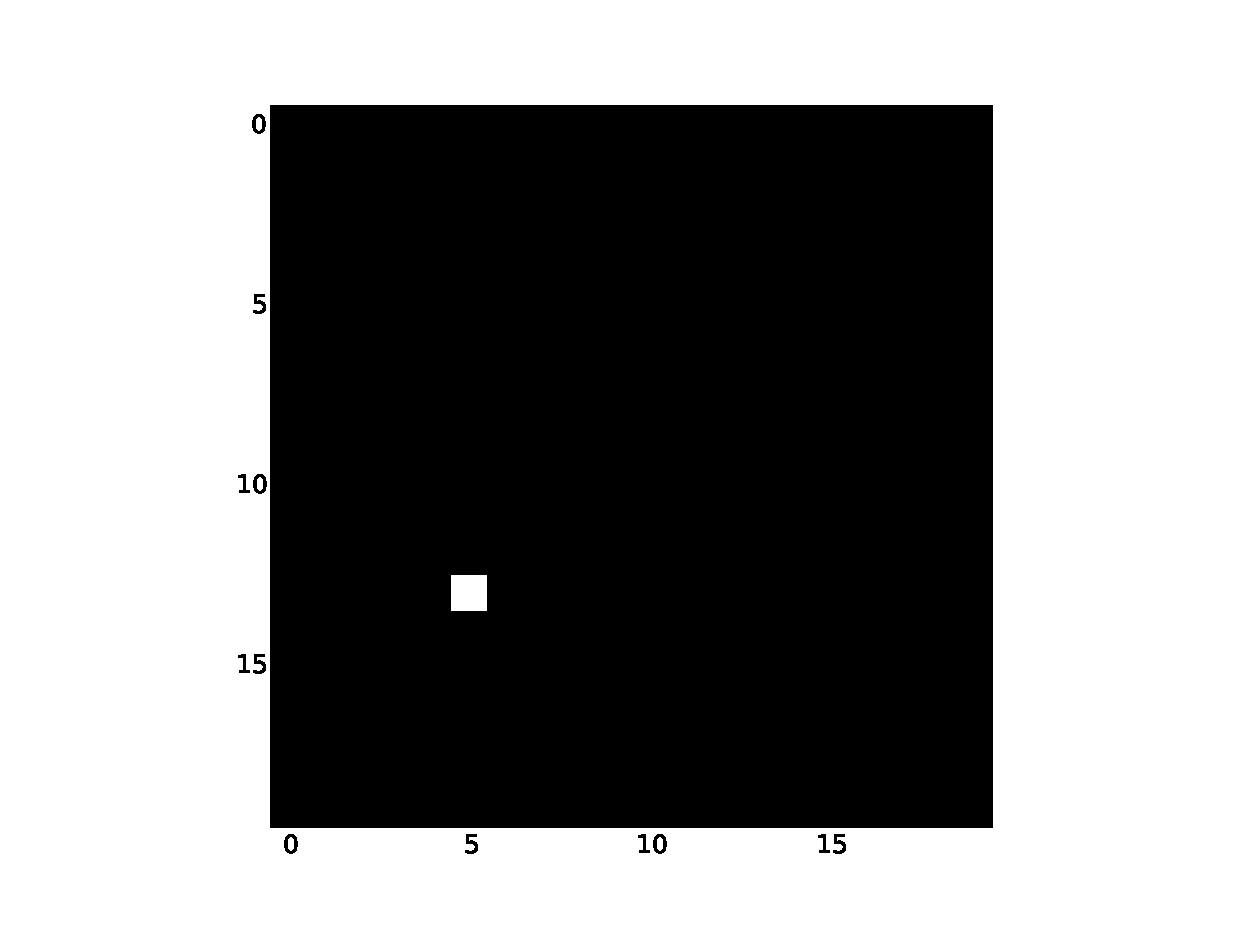
\includegraphics[width=0.3\linewidth]{fig/20/15.eps}
\label{fig:s15}
}

\label{fig:ising_states}
\caption{The final states of the 2D Ising spin systems for different $ \beta $.}
\end{figure}


The phase change at around $ \beta= 0.44 $ is evident. The exact calculation of the critical temperature was achieved by analytical means by Onsager. \cite{onsager} The critical temperature is calculated via this condition

 \begin{equation}
 2 \tan^2 \left( 2\beta_c J \right) = 1
  \end{equation}
  
Which in our case predicts a critical temperature of $ \beta_c = 0.4405 $ in agreement with the results. 

A very simple change that gives one the chance when this modular approach is taken is that when the elements, the definition of the spins and energy are changed, the whole code remains intact, since the core of the code applied to any system with an ensemble and energy definition. 

One may change the definition of a spin, a spin that may take one the values from $ \lbrace -1,-0.5,0,0.5,1\rbrace  $. This results in a different system, and one should update the Metropolis algorithm such that it encompasses systems of multiple energy levels. The algorithm may be updated such that if for one of the spins, there exists a lower energy configuration, than the system takes the state with the lowest of those energies. If the system is in the lowest energy configuration,  then the next state it is going to be in is determined by the probabilities determined by the Boltzmann distribution as it was in the case of Ising spins. This system is ran within a grid of $ 15 \times 15 $, the macroscopic parameters are calculated accordingly. 


\begin{figure}[H]
\center
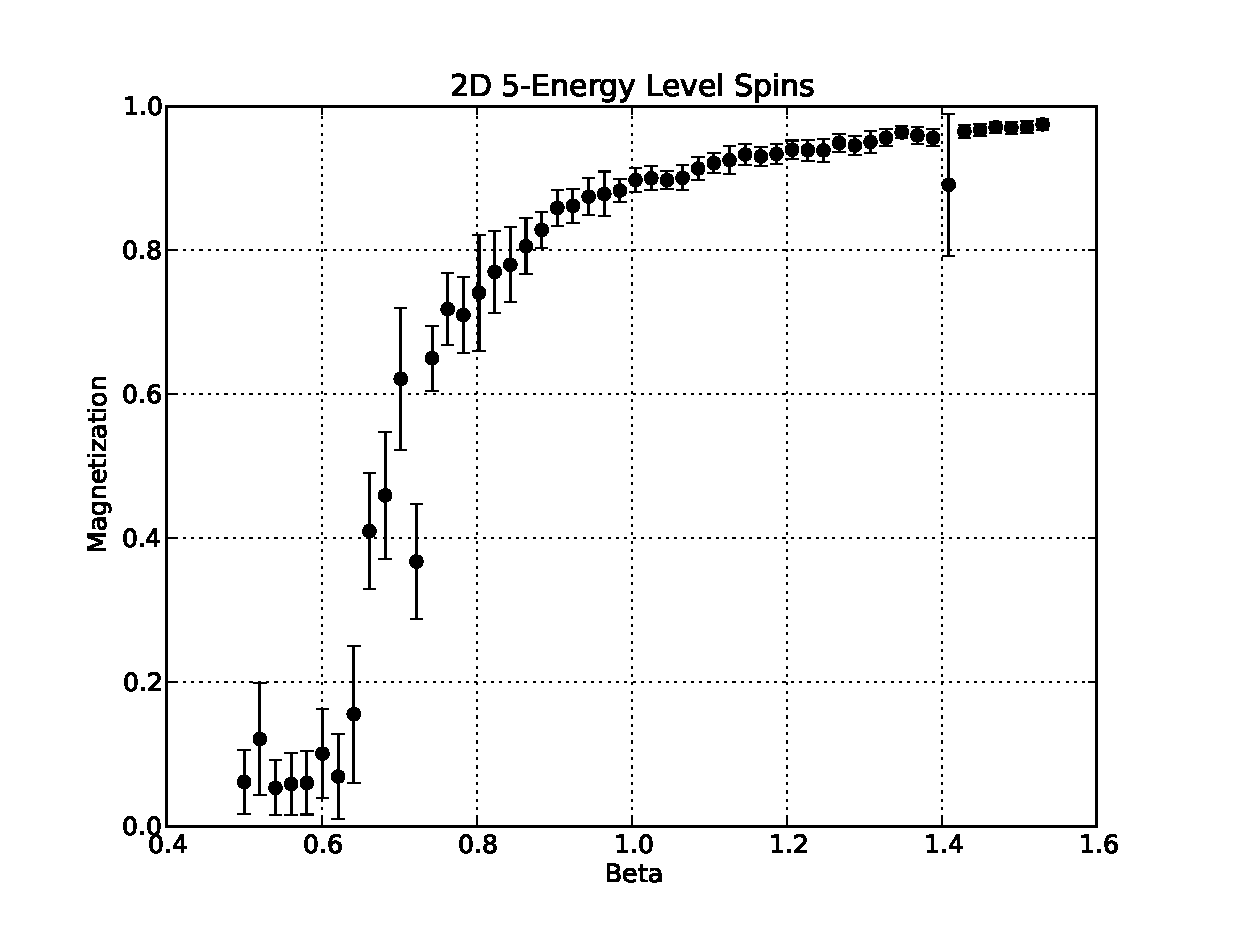
\includegraphics[width=\linewidth]{fig/15/plot.eps}
\label{fig:225spins}
\caption[The dependence of magnetization $ M $ due to the temperature, $ \beta $ in 5-level spins.]{The dependence of magnetization $ M $ due to the temperature, $ \beta $. The error bars correspond to the standard deviations and the dots correspond to the mean of the data set taken for that $ \beta $ value. The deviations from the orderly phase are from the fact that the standard deviation may turn out to be low though the algorithm hadn't converged.}
\end{figure}

\begin{figure}[ht]
\centering
\subfigure[$ \beta=0.1 $]{
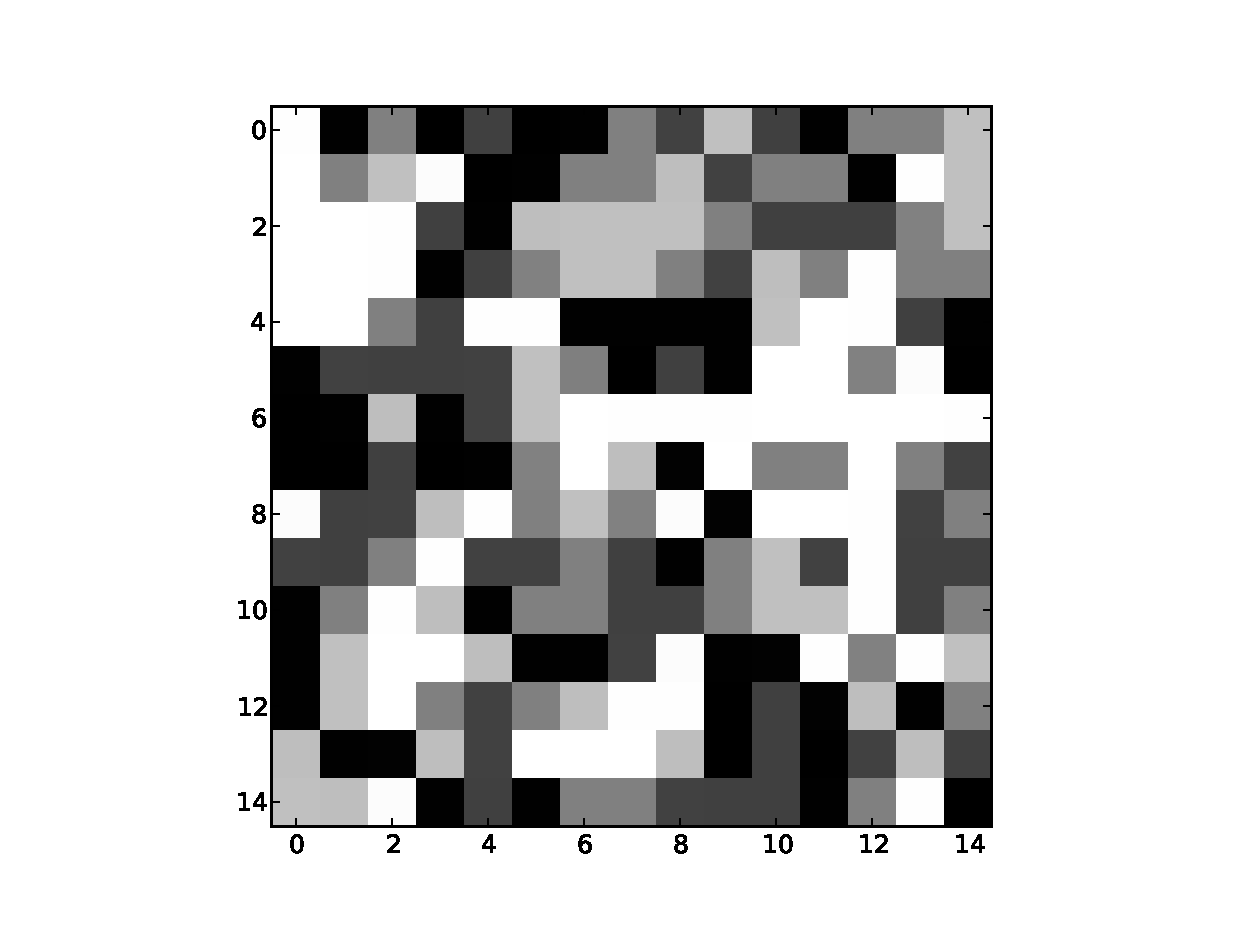
\includegraphics[width=0.3\linewidth]{fig/15/1.eps}
\label{fig:s51}
}
\subfigure[$ \beta=0.15 $]{
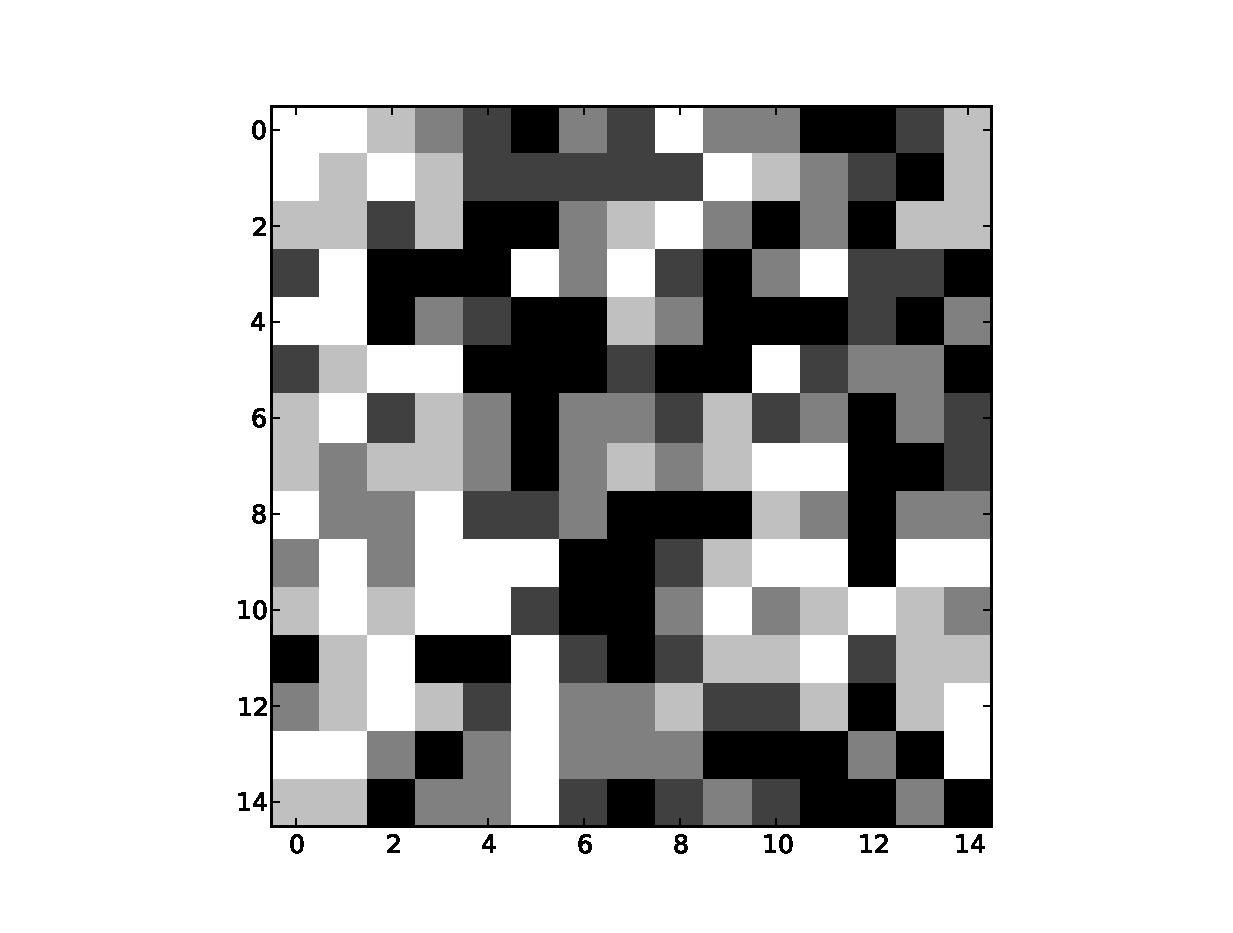
\includegraphics[width=0.3\linewidth]{fig/15/2.eps}
\label{fig:s52}
}
\subfigure[$ \beta=0.2 $]{
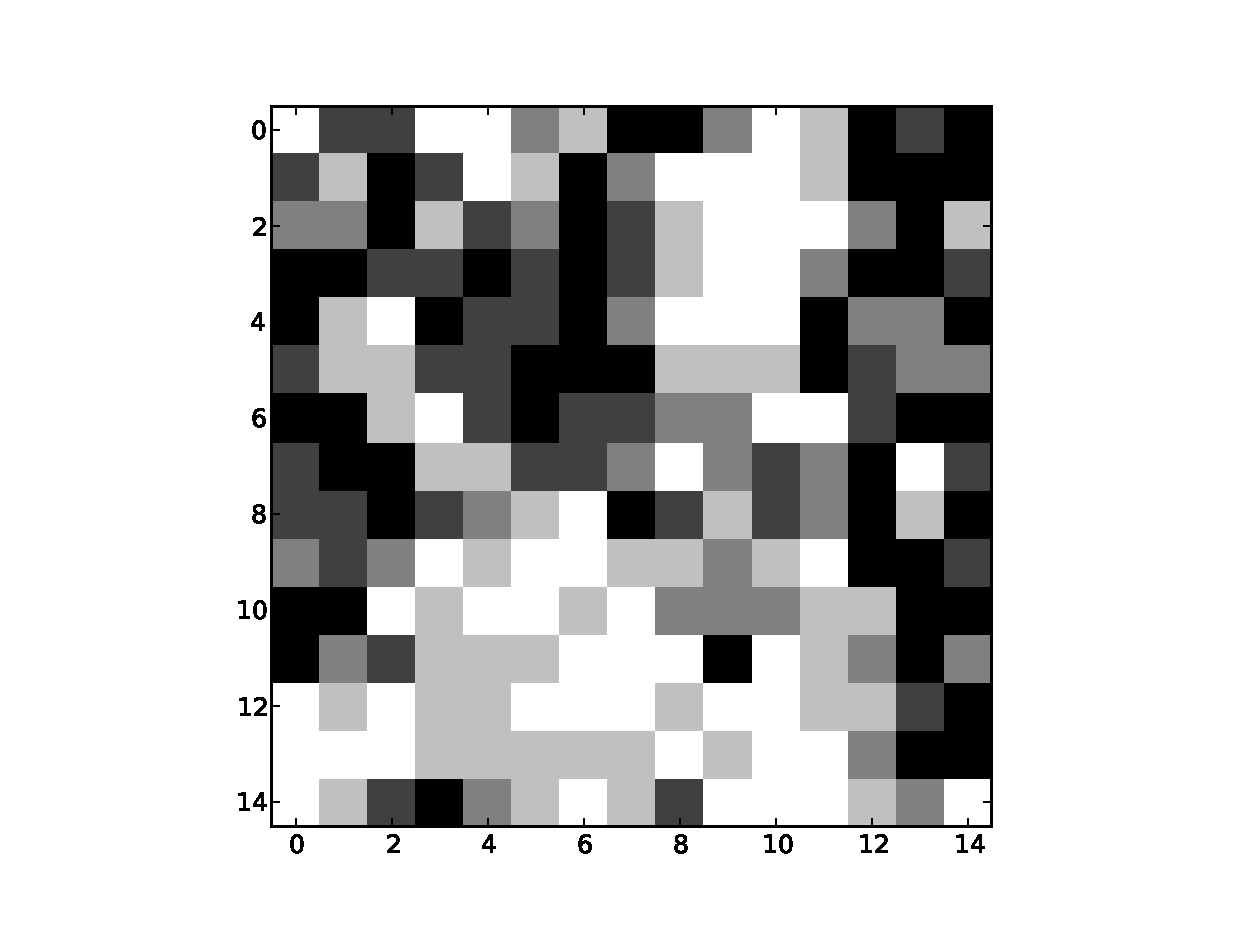
\includegraphics[width=0.3\linewidth]{fig/15/3.eps}
\label{fig:s53}
}
\\
\subfigure[$ \beta=0.25 $]{
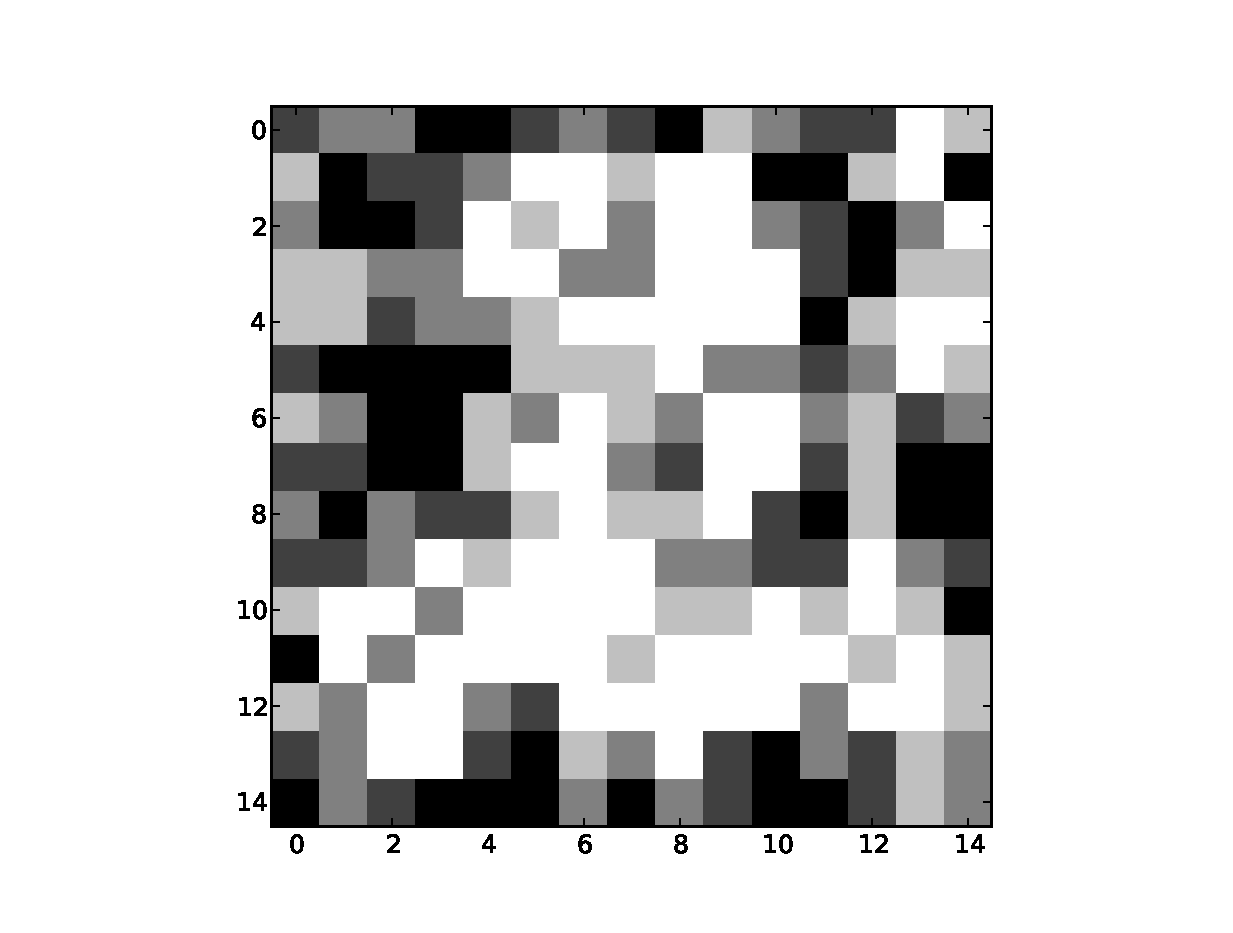
\includegraphics[width=0.3\linewidth]{fig/15/4.eps}
\label{fig:s54}
}
\subfigure[$ \beta=0.30$]{
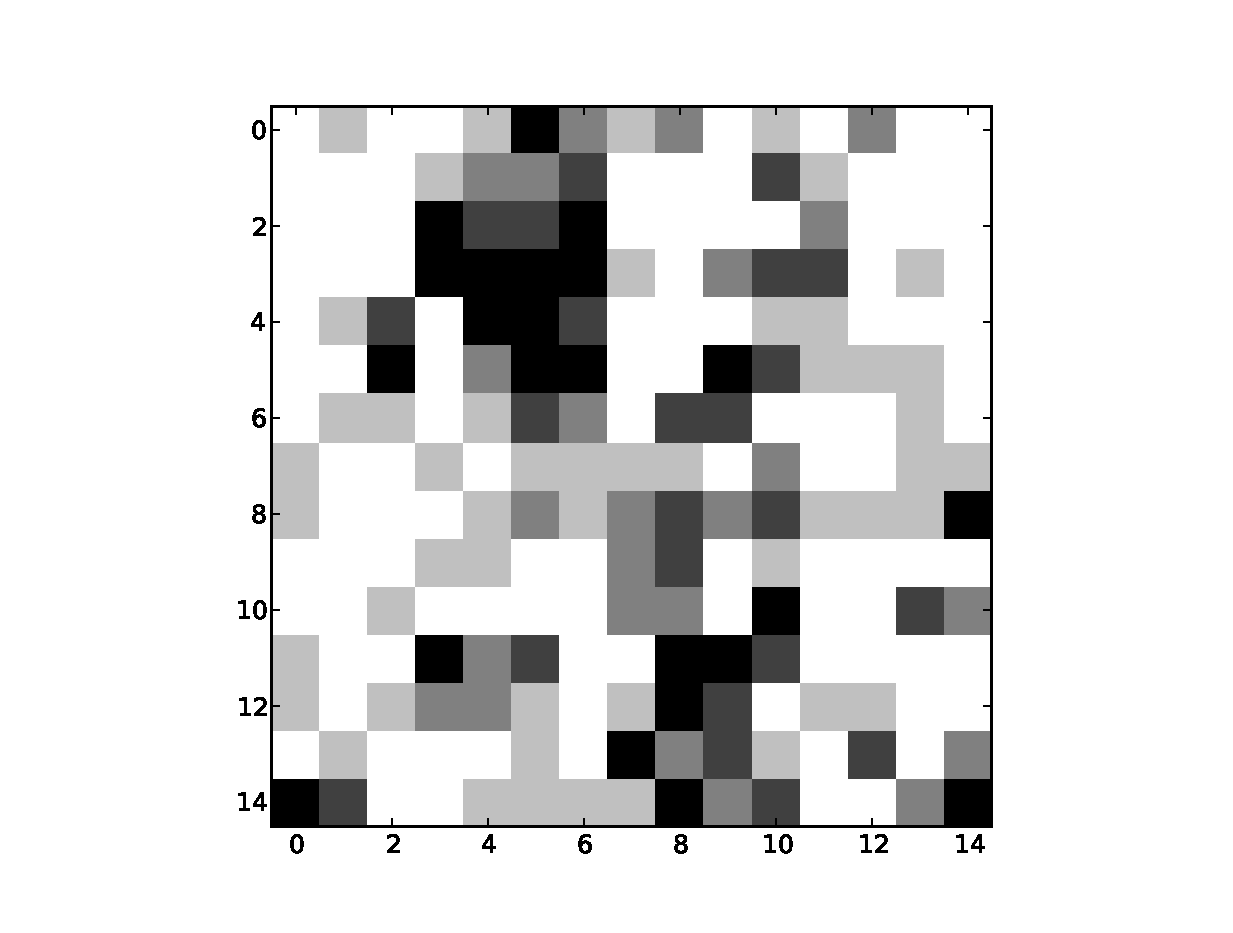
\includegraphics[width=0.3\linewidth]{fig/15/5.eps}
\label{fig:s55}
}
\subfigure[$ \beta=0.35$]{
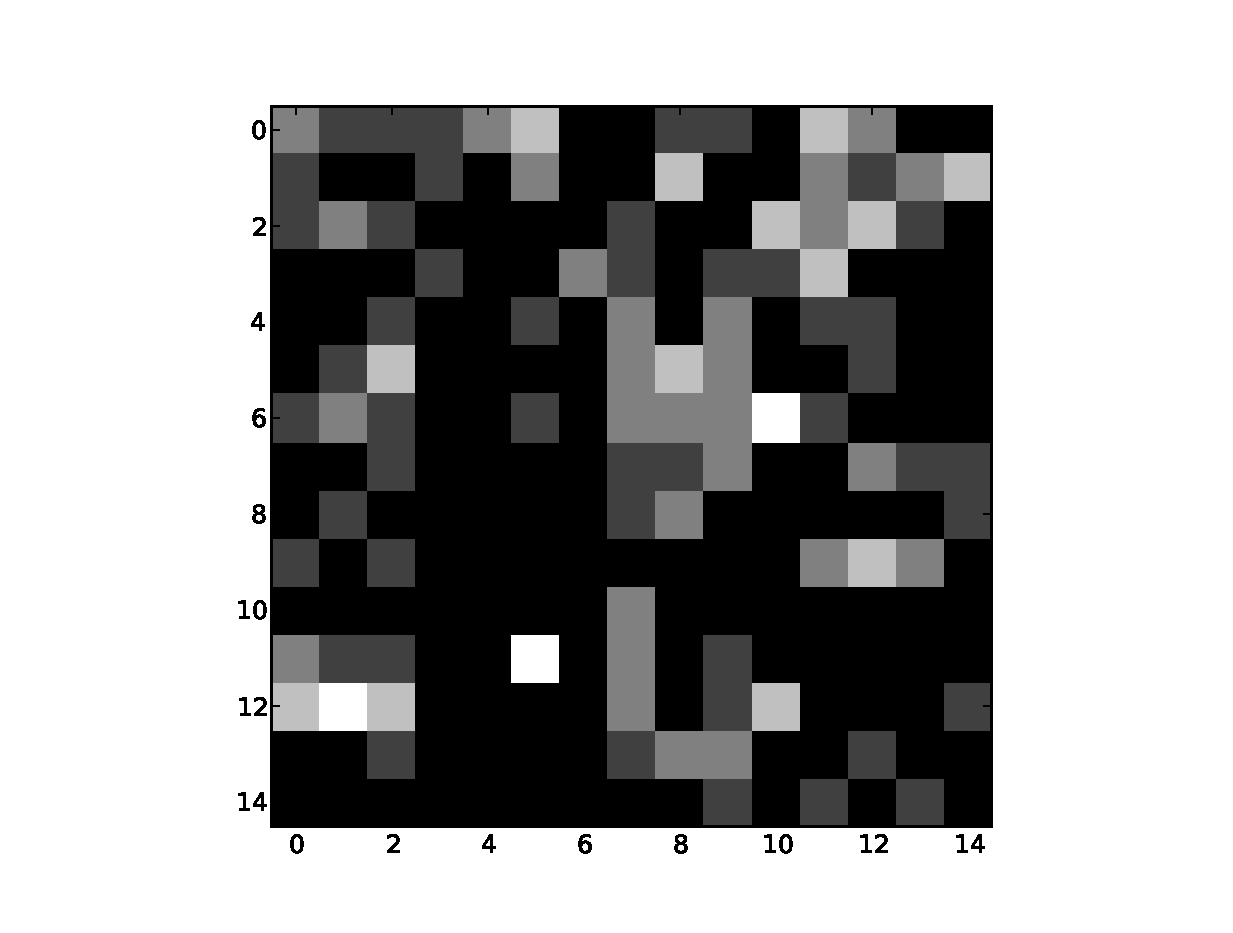
\includegraphics[width=0.3\linewidth]{fig/15/6.eps}
\label{fig:s56}
}\\

\subfigure[$ \beta=0.40$]{
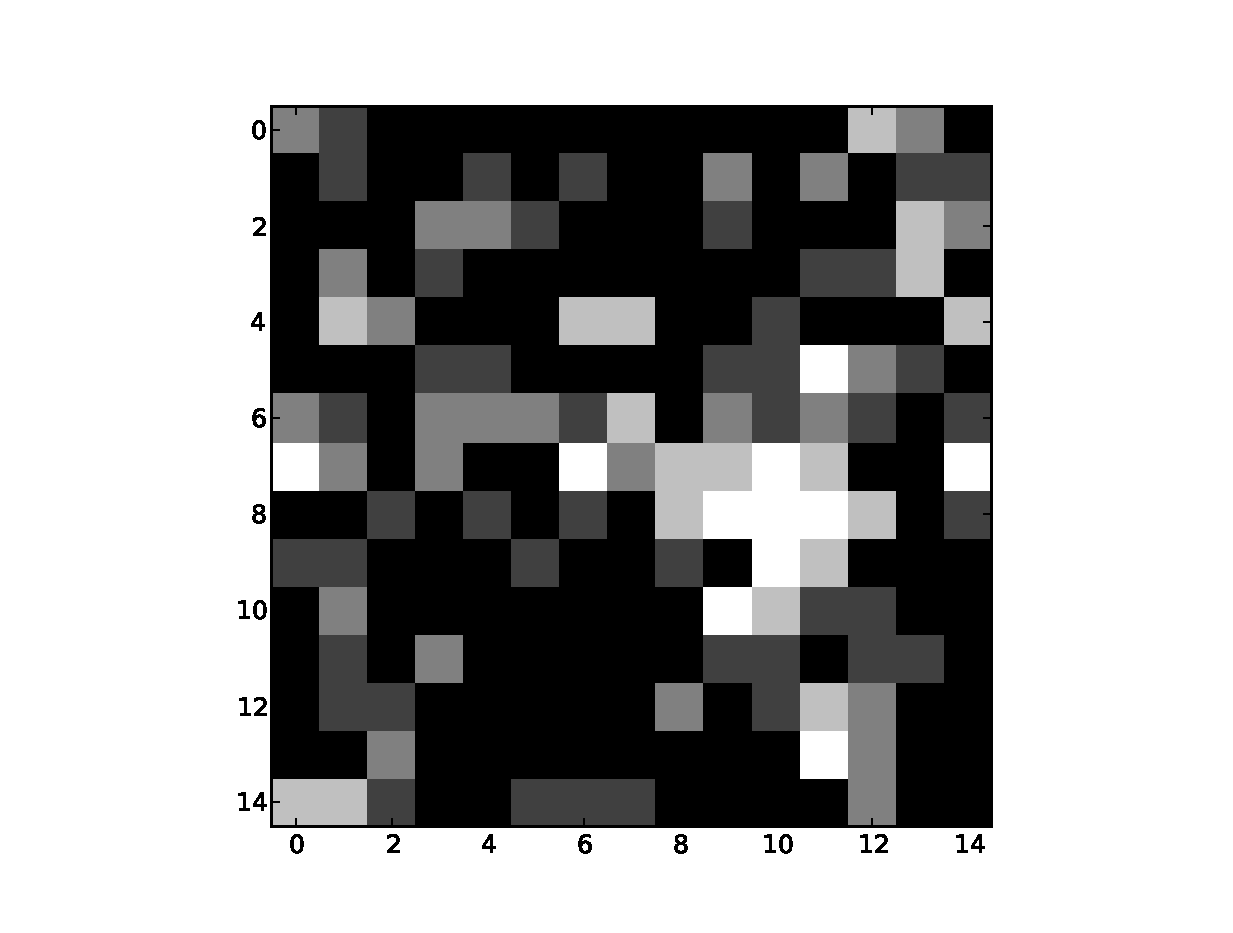
\includegraphics[width=0.3\linewidth]{fig/15/7.eps}
\label{fig:s57}
}
\subfigure[$ \beta=0.45 $]{
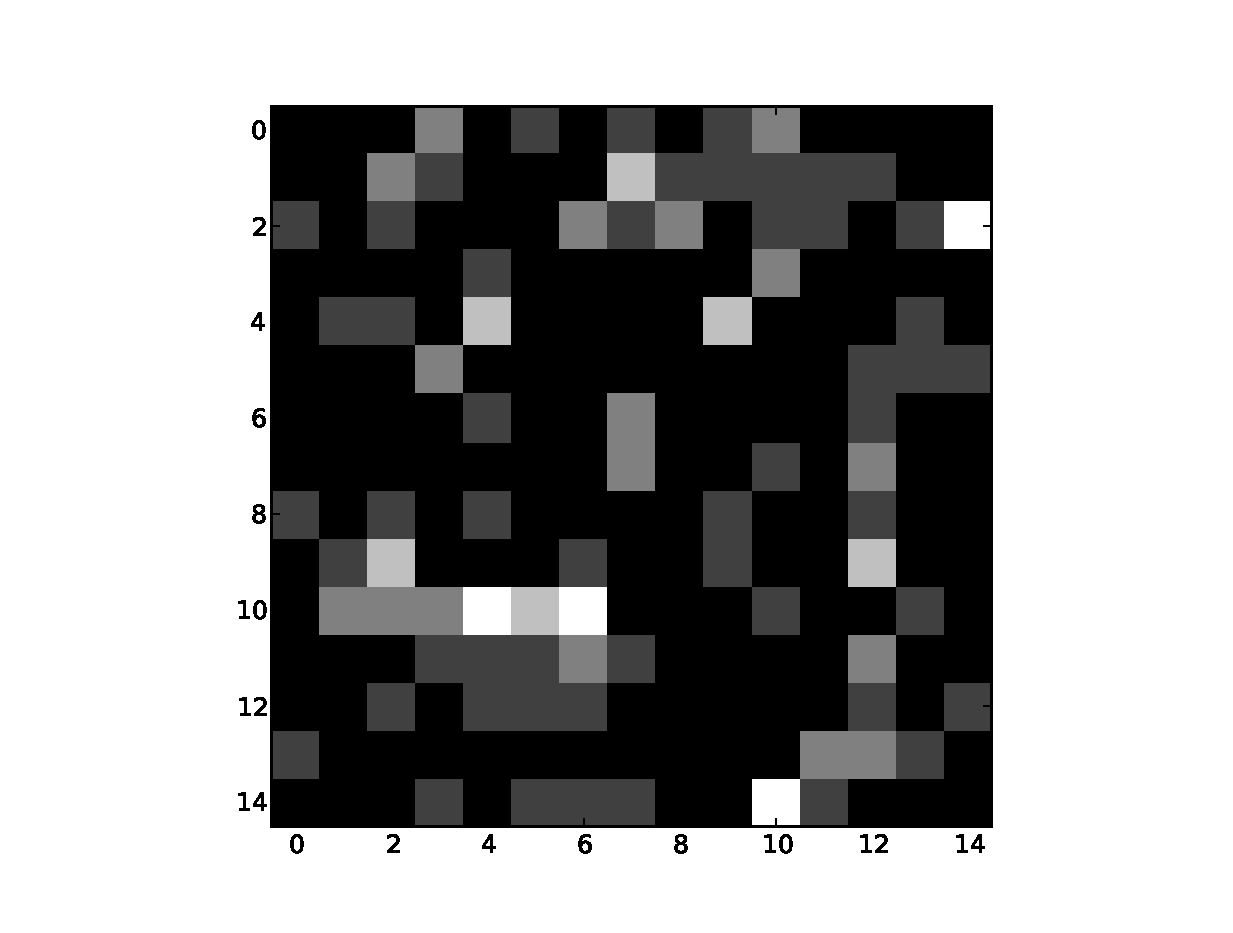
\includegraphics[width=0.3\linewidth]{fig/15/8.eps}
\label{fig:s58}
}
\subfigure[$ \beta=0.50$]{
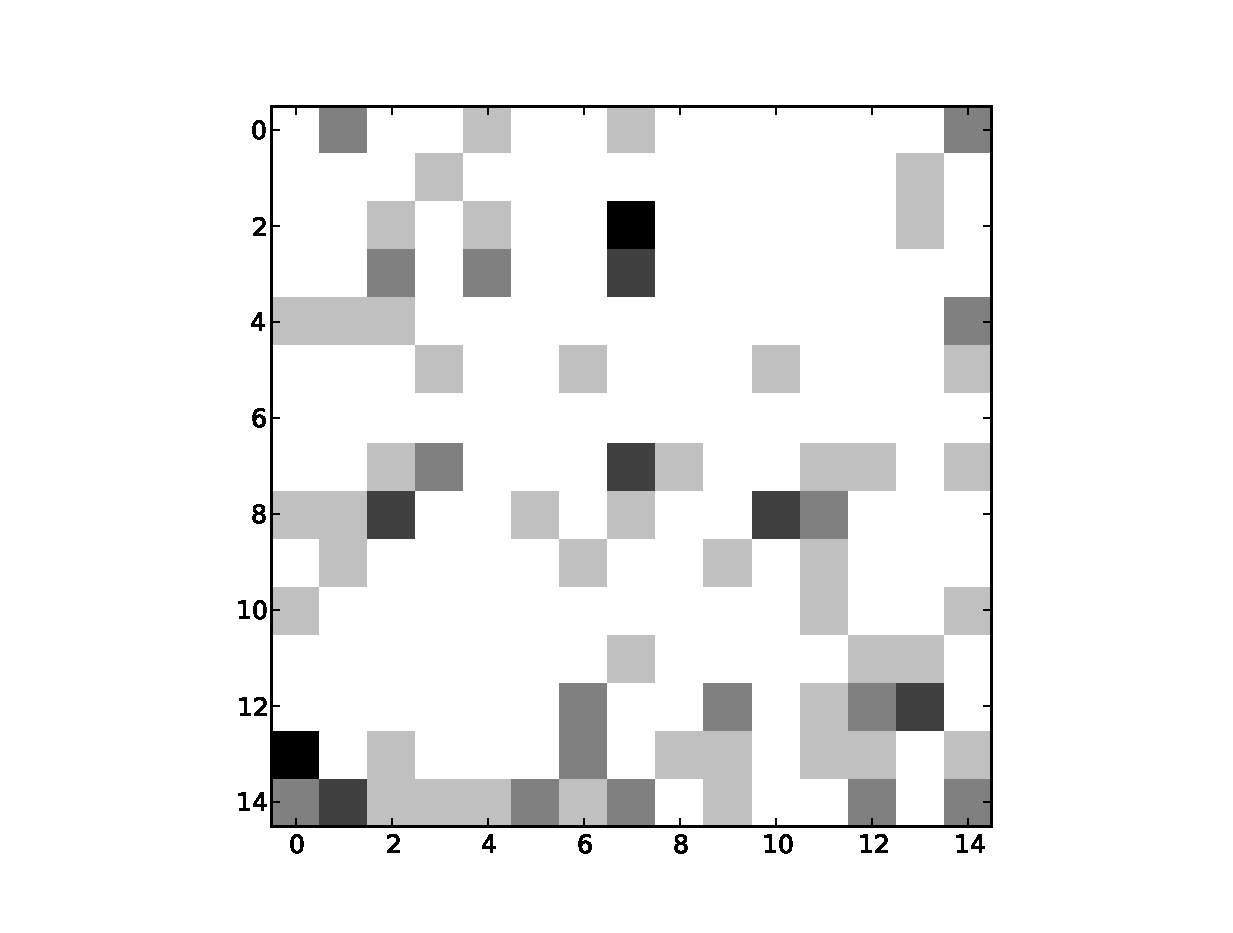
\includegraphics[width=0.3\linewidth]{fig/15/9.eps}
\label{fig:s59}
}\\

\subfigure[$ \beta=0.55$]{
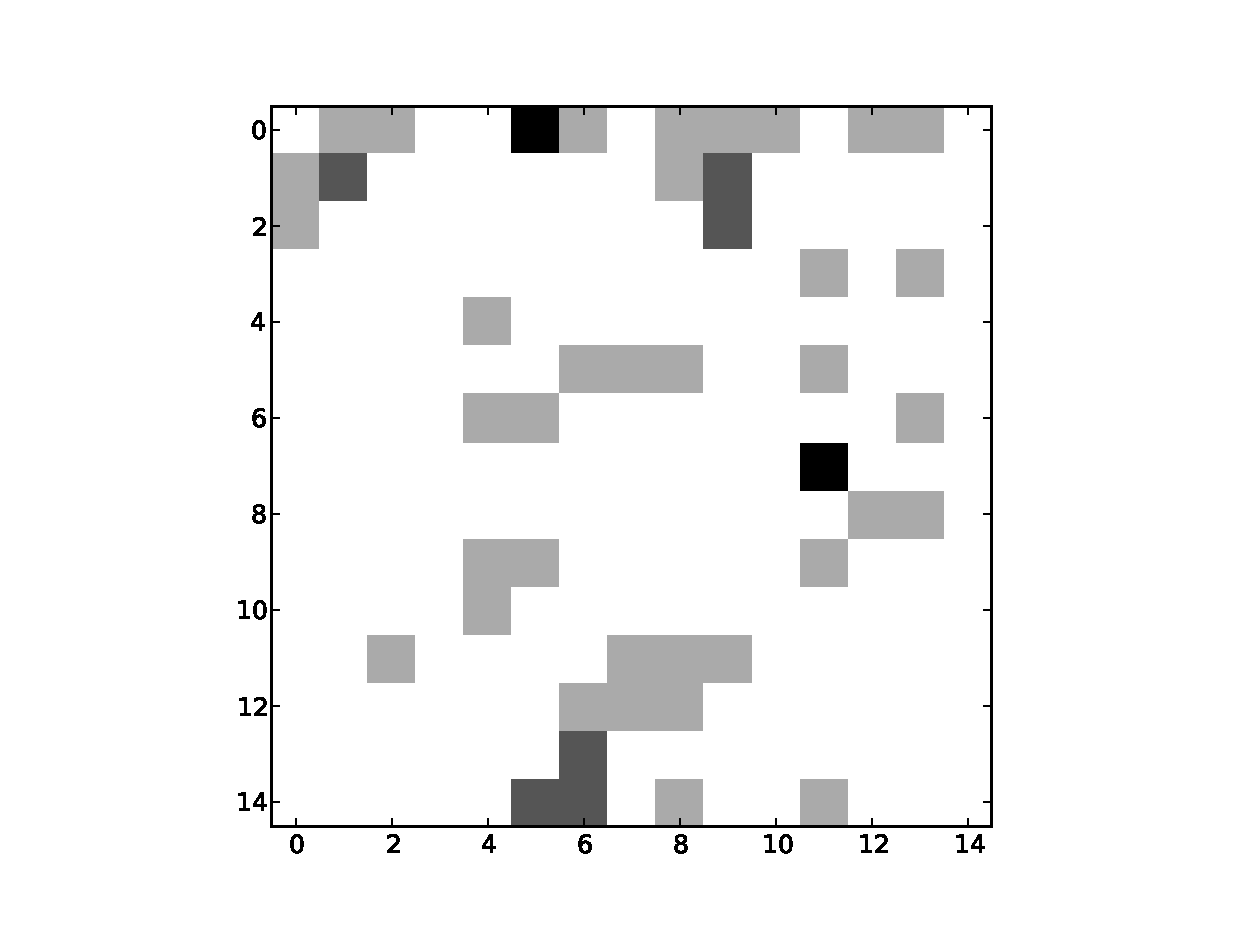
\includegraphics[width=0.3\linewidth]{fig/15/10.eps}
\label{fig:s510}
}
\subfigure[$ \beta=0.60$]{
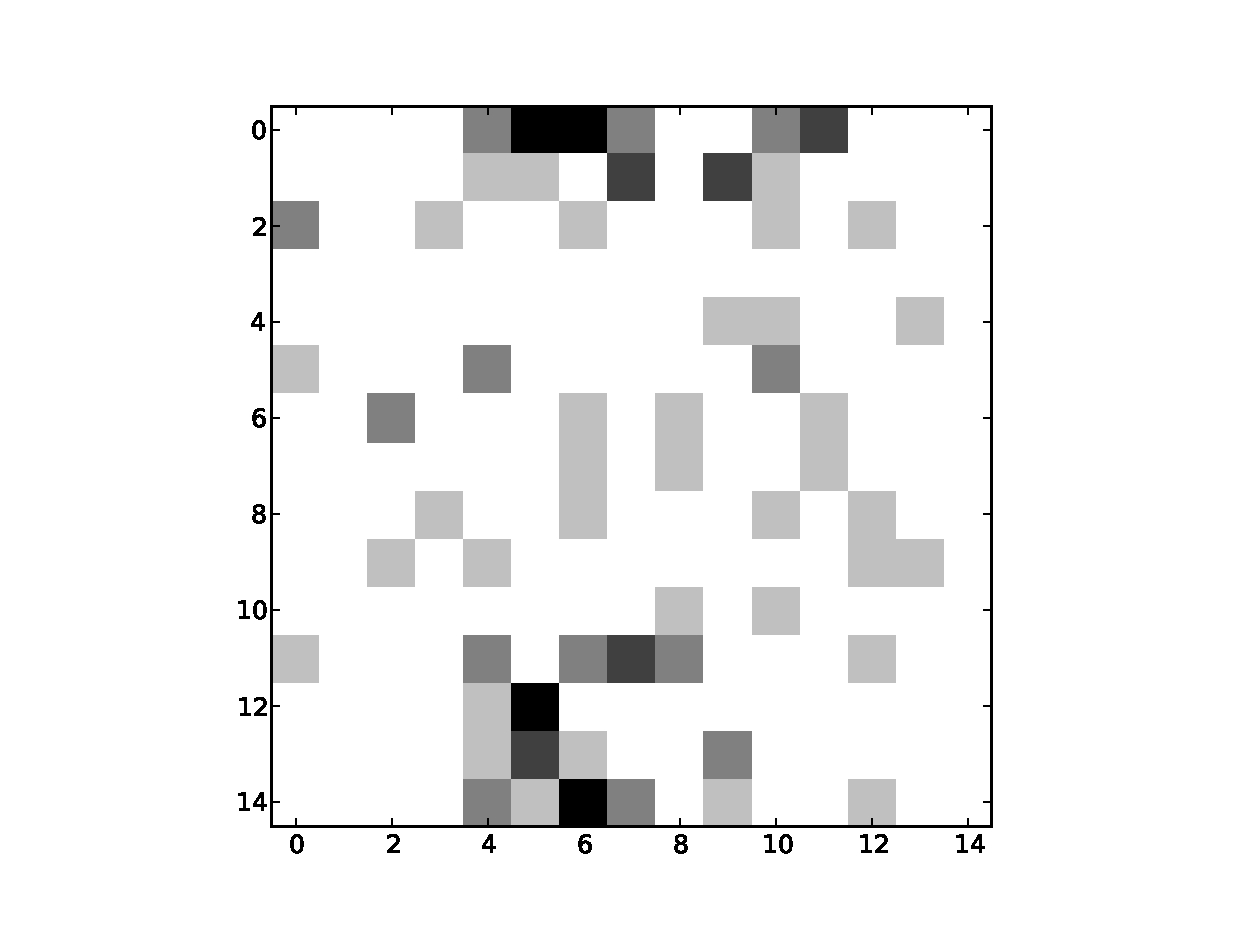
\includegraphics[width=0.3\linewidth]{fig/15/11.eps}
\label{fig:s511}
}
\subfigure[$ \beta=0.65$]{
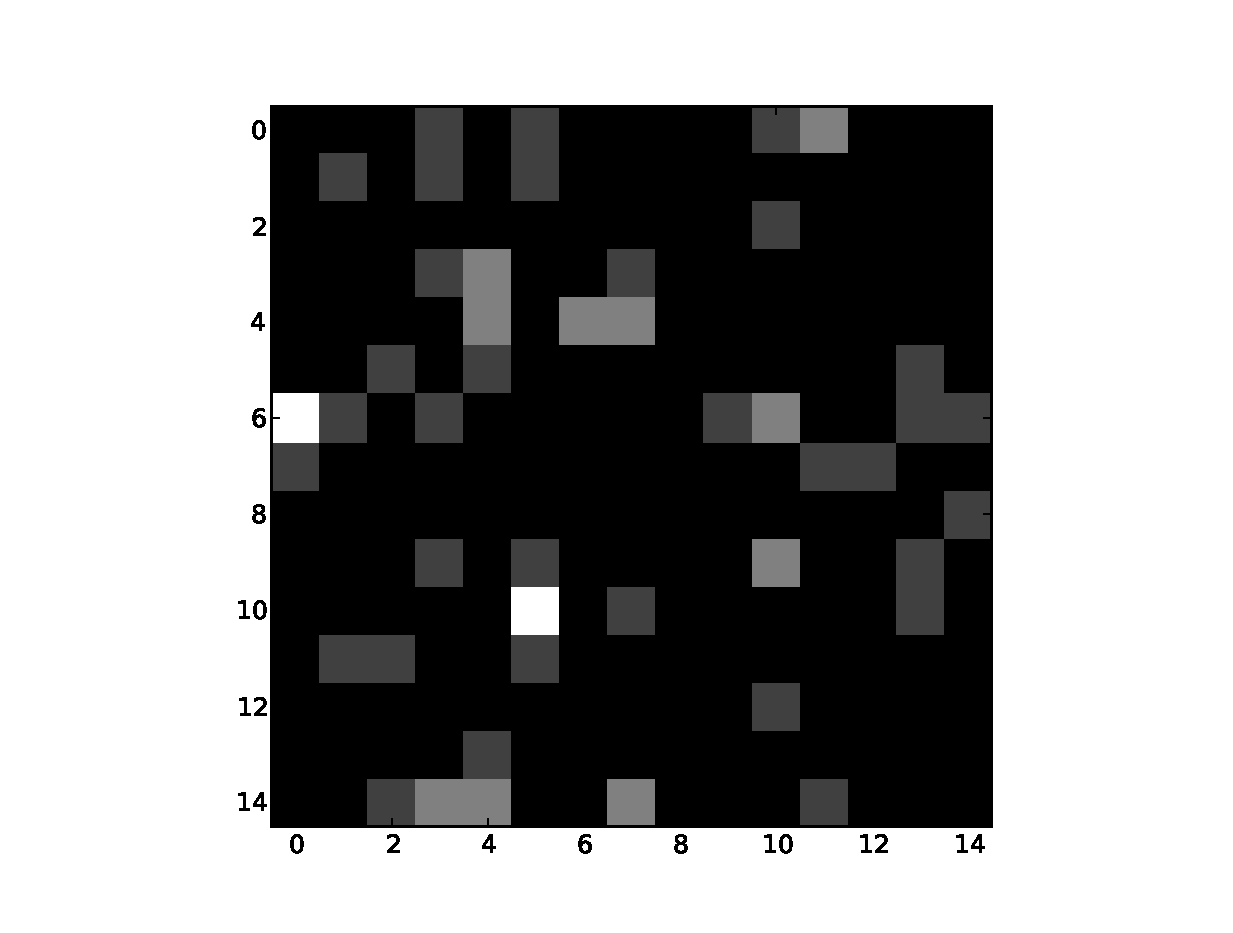
\includegraphics[width=0.3\linewidth]{fig/15/12.eps}
\label{fig:s512}
}\\

\label{fig:5ising_states}
\caption{The final states of the modified 2D Ising spin systems for different $ \beta $.}
\end{figure}

The phase change is more gradual, and now, the critical temperature is higher, $ \beta_c \approxeq 0.7 $.

\section{Protein folding}
In order to get out of the world of spins, one might come up with different systems, such as a system where a protein is made out of kinks that interact with Coulomb potential. The simulation for such system is in progress, but didn't finish at the time when this report was being written. Though, the process is similar. The Monte Carlo algorithm is changed in a way that the ensemble is a long 30-piece chain of pieces of same length, with corners randomly selected to be positively charged, negatively charged, or neutral. The perturbation is a small change in angle between two consecutive chains. The energy is the Coulomb potential of this arrangement of charges. Though the proteins could be visualized to be  folding, some problems arise from the floating point precision. 

\begin{figure}[H]
\center
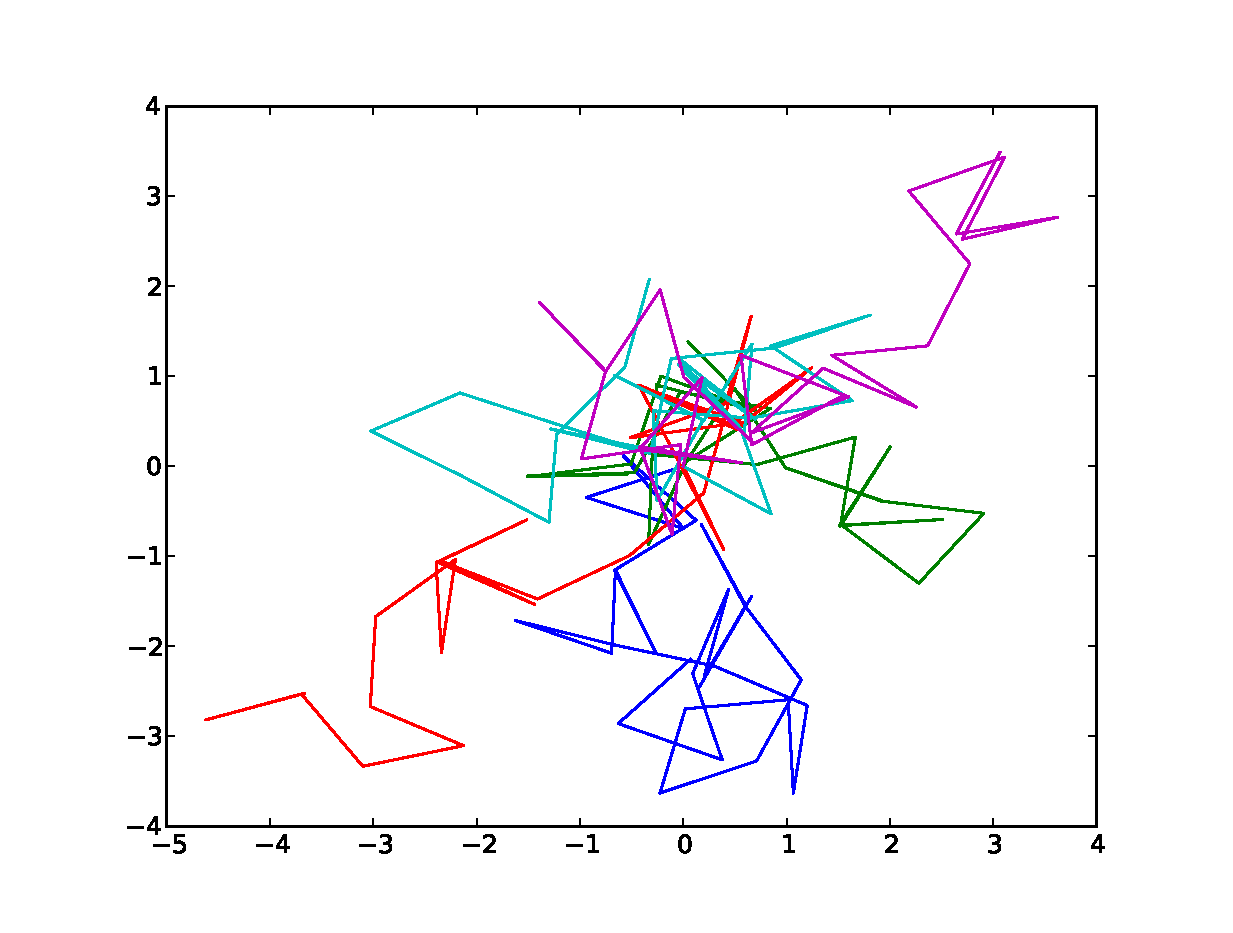
\includegraphics[width=\linewidth]{fig/kink/384242424242.eps}
\label{fig:kink}
\caption{Several chains that the algorithm converged. In these chains, $ \beta \cong 3.9 $, in hotter environments, the chains fail to satisfy the convergence criteria. }
\end{figure}


\section{The Code Used for this Project}

The code used in this project is named as \emph{Monty Carlo} and is available as Git repository. ın order to have a copy, contribute to the code, please copy the repository with the command:

\begin{lstlisting}[language=bash]
git clone git://github.com/mehmetalianil/monty-carlo.git
\end{lstlisting} 

This will create a folder and put the source code as it was on my pc when I commited my changes to the project. When there is an update, this update can be downloaded via the command:

\begin{lstlisting}[language=bash]
git pull origin
\end{lstlisting}

If one has made a change to the source code on his/her computer, than that copy becomes a fork of my project, in order to maintain the simultaneity of these two copies, these changes must be merged together. Contact me via \emph{mehmet.ali.anil@ieee.org} if you want to contribute to the code. 
